\graphicspath{{images/}}
% 3.  Descrizione della piattaforma
\chapter{The Data Entry Tool}
The Data Entry Tool is part of an enterprise customer's digital transformation, consisting of a robust and integrated solution that enables the coexistence and interoperability of on-premise, private and public cloud data resources. The required platform guarantees access to and manipulation of data from multiple sources offering on-demand requests in near real-time. It will be the tool's job to validate and redirect the data to the corresponding database, as well as grant a user the access only to a subset of tables, according to the given permissions.

\section{Requirements}
% 3.1  Requisiti  (es. tipologie di utenti, funzionalità quali aggiunta DB/gestione privilegi/gestione audit...)
The requirement for the tool were the following:
\begin{itemize}
    \item There has to be a distinction between a normal User and an Administrator of the Data Entry Tool;
    \item Tables can insist on several databases and the supported engine are PostgreSQL, Oracle, and MSSQL Server;
    \item Tables can be organized in groups in such a way as to create a 2-level depth hierarchy;
    \item Each table could be assigned an action in JSON format that would be performed on-demand;
    \item A subset of permissions is assigned to each table, spanning from simple visualization to direct alteration of values;
    \item Permissions to users are provided by creating associations between groups of users and a table or groups of tables;
    \item Each Field in a table is associated with a data type which will help its validation;
    \item The possibility of importing/exporting data from/to Excel files must be arranged;
    \item Each operation performed by a User must be tracked.
\end{itemize}


\section{Architecture}
% 3.2  Architettura  (evidenziando quali moduli funzionali ha sviluppato lei, e i loro servizi)
The overall architecture is composed by three different elements: the underlying database of the tool, the Back-End, and the Front-End, as seen in Figure \ref{fig:CompleteArch}.
Firstly, the database allows to map an existing database that belongs to the client; this database could be located anywhere, either in the cloud or on-premise, as long as it is reachable via the AWS subnet. This is where all users of the tool are registered, with the respective permissions on each table, as well as a set of logs regarding all the operation performed by any of them. 

\begin{figure}[!htb]
    \centering
    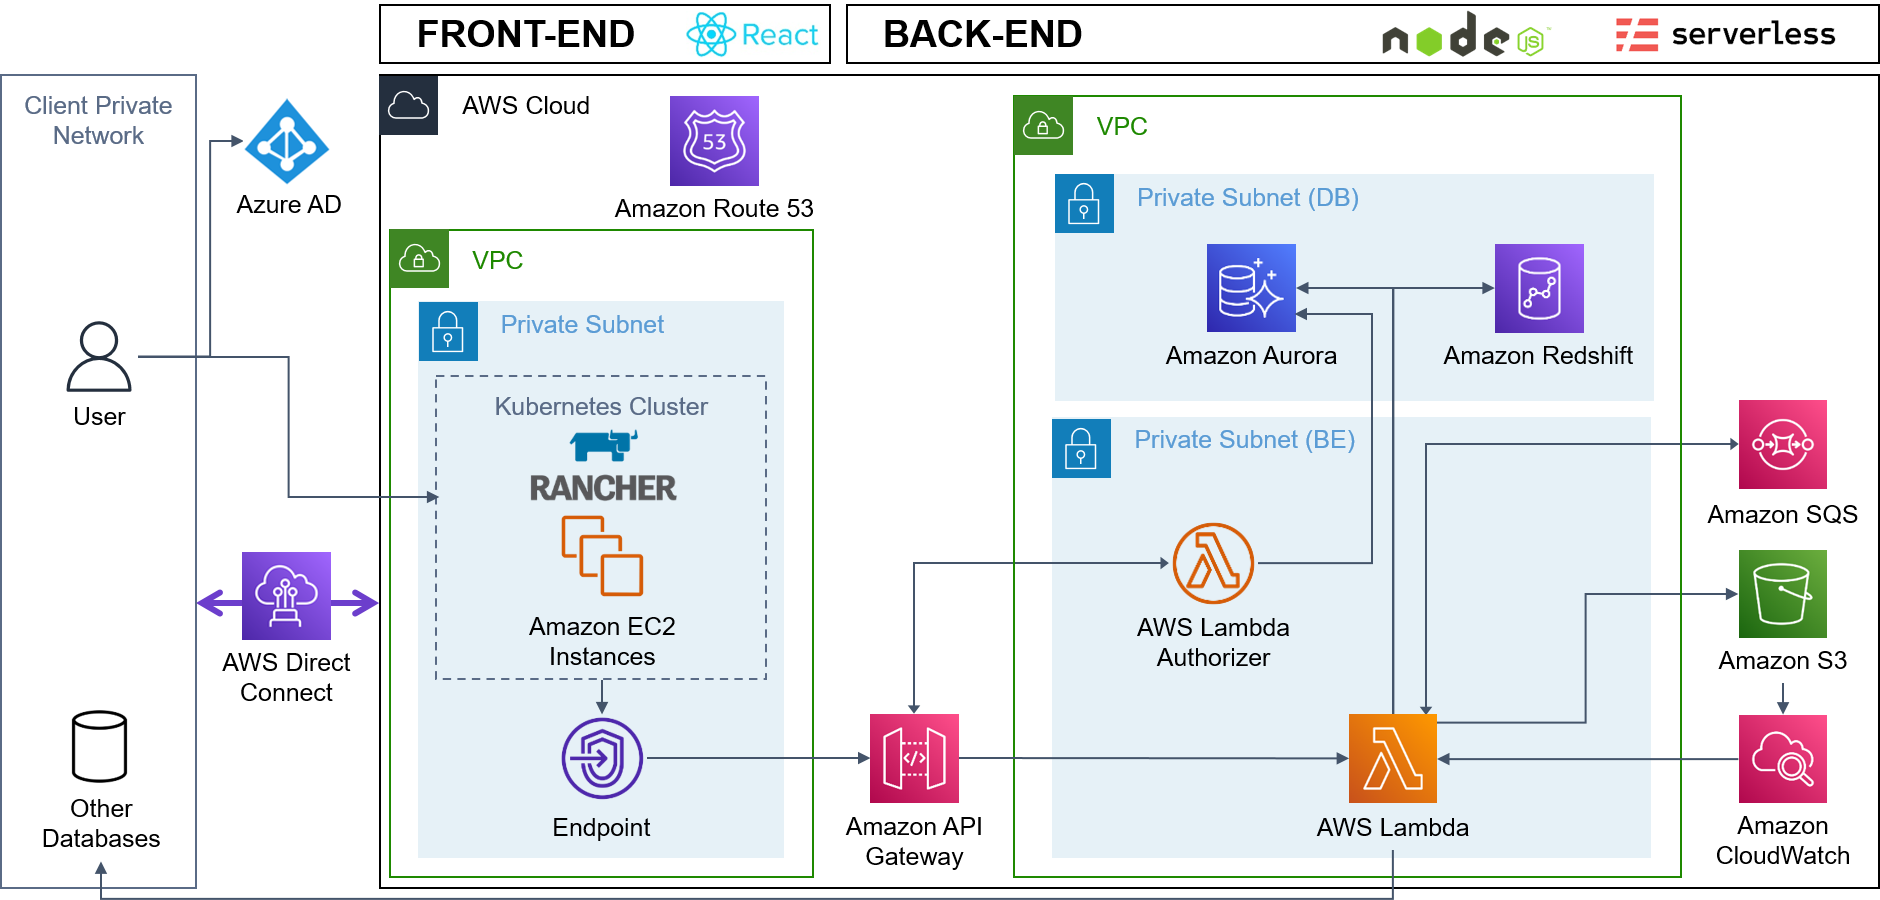
\includegraphics[width=15.8cm]{chapters/images/ch_3/CompleteArch.png}
    \caption{High level overview of the Data Entry Tool.}
    \label{fig:CompleteArch}
\end{figure}

Then, the Back-End contains all the logic regarding database mapping, the inclusion, authentication, and authorization of the users, the granting and revoking of the permissions, external tables manipulation and data validation, and the logging of all operations.

Finally, the Front-End is where users and administrators interact with all registered databases:
an administrator insert new users, databases, and tables, and creates associations between users and tables with all the required permissions; 
a user performs operations on the permitted tables without any knowledge to where they are stored or which underlying database is working with, all with an homogeneous view for all the tables.

As part of my work, I was involved in the design of the whole architecture and the development of the Database, Back-End, Front-End, and CI/CD aspects.

\subsection{Database}
The DBMS chosen to handle the tool-related data is an instance of Amazon Aurora PostgreSQL.
For the versioning of the database schema we used Flyway, which, as said before, is a tool that performs database migrations. To make use of it in the CI/CD pipeline, I leveraged the available docker image and created a docker compose file which, by automatically obtaining the connection parameters from the environment variables and mapping the SQL versioning files, performs the migrations of the schema. 


\begin{figure}[!htb]
    \centering
    \includesvg[inkscapelatex=false, width = 15.8cm]{ch_3/ER-Schema}
    \caption{Entity-Relationship Schema}
    \label{fig:ER}
\end{figure}

In the ER Schema in Figure \ref{fig:ER}, we can see all the elements used to map a database in the tool, as well as handling of the authentications and authorizations to perform operations.
\begin{itemize}
    \item \textbf{Users}: an entity who represents the users of the Data Entry Tool; they can be differentiated in normal user and administrator, where the administrators are a subset of all the users, which means that they can also utilize the tool as normal users do.
    
    \item \textbf{Audit Log}: all the operations carried out by users are registered here; each log contains on which table it was performed, the type of the operation, the status, the data used and eventual errors, and when it was performed.
    
    \item \textbf{Databases}: this table contains the connection parameters for each database that the tool has to manage.
    
    \item \textbf{Tables}: here all the tables of all the registered databases are gathered; each one contains the original name of the schema and table in the respective database. Also, a table may contain the definition of an action that is performed upon request of the user.
    
    \item \textbf{Table Fields}: this table contains all the column of a table in a given database. Each field maintain the details of a column, from the constraints like being a primary key column to the data type, from a list of possible values to the maximum number of chars that constitute it. There is also the possibility to set features for each field:
    \begin{itemize}
        \item \emph{Primary Key}: marks a field as Primary Key; multiple fields can be Primary Key;
        \item \emph{Is Required}: the user has to provide a value for this field;
        \item \emph{Visible}: sets the field as visible by the user that views the table;
        \item \emph{Editable}: makes the field editable by the user;
        \item \emph{Sortable}: Allows the user to sort the table according to this field;
        \item \emph{Filterable}: Allows the user to filter the table according to this field;
        \item \emph{Fixed Column}: does not allow the column to move during horizontal scroll of the table;
        \item Note: the distinction between the ``\emph{Primary Key}'' and the ``\emph{Is Required}'' features is due to the fact that a primary key may not be required; as an example, consider an auto-increment primary key: in this case, the user should not be allowed to manually enter a value as it would cause inconsistency in the database.
    \end{itemize}
    
    \item \textbf{Table Collections}: collections are a way of aggregating tables and displaying them to the user in an orderly fashion. Only tables that are included in a collection will be shown to users.
    
    \item \textbf{Tables Import Export}: this table contains all the import and export operations  with the relative status.
    
    \item \textbf{User Groups}: Each user group contains the association between users and tables (N-to-M); these associations tell a user which tables are visible and what kind of manipulation s/he can perform on them. If a User has access to the same table through distinct groups, the sum of the permissions given to each group would be granted. E.g. if group A gives users the ability to delete data in table X, and group B the ability to insert new data in X, then the users that are part of both group A and B will be granted the ability to delete and insert data in X.
\end{itemize}


To speed up data retrieval from this database, we have created views and indexes. 

% \clearpage

\subsection{Back-End}
The aforementioned database represents the state of the tool, while the Back-End represents the stateless part. Here, through the Amazon API Gateway, all the functions that manipulate the tool database and all the external ones can be called with a specific REST API. Moreover, many APIs also use something called \emph{Path Parameters} and \emph{Query Parameters}. Path parameters are variable parts of a URL path. They are used to point to a specific resource within a collection, such as a user group identified by an ID. A URL can have several path parameters, each indicated by curly brackets. Query parameters on the other hand are key-value pairs that are an optional part of the path and are primarily used to perform the sorting, pagination and filtering of the tables from the Back-End side.

\begin{figure}[!htb]
    \centering
    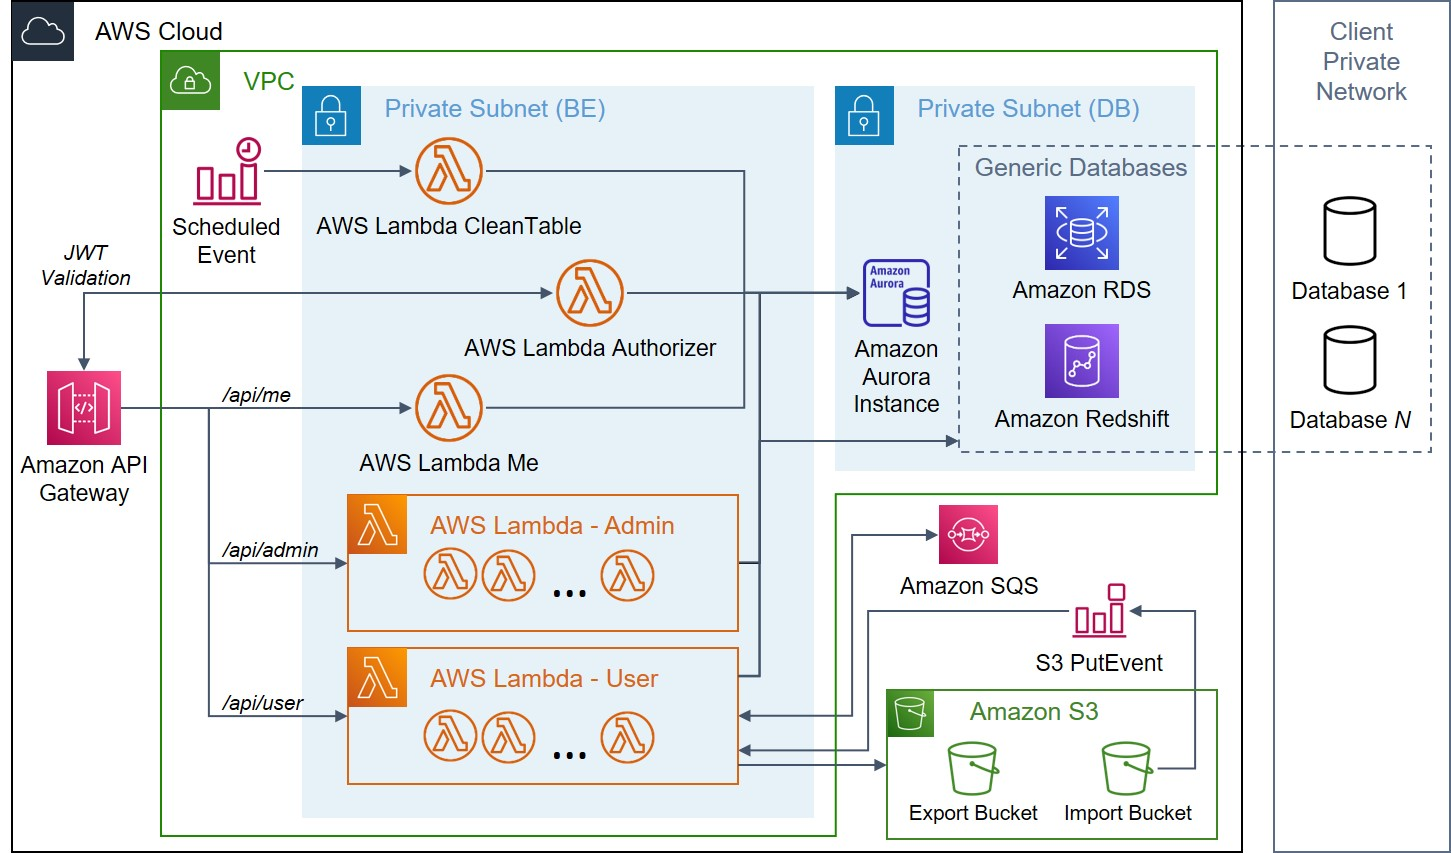
\includegraphics[width=15.8cm]{chapters/images/ch_3/BE_Common.jpg}
    \caption{High level overview of the Back-End architecture.}
    \label{fig:BE_Common}
\end{figure}

As we can see in Figure \ref{fig:BE_Common}, before performing any operations on the tool, any user who is logging in, whether an administrator or a user, will be authenticated and authorized by the \emph{Lambda Authorizer} to perform specific operations on the tool. Some Lambdas are also used to perform scheduled cleaning of tables used as support for certain operations.

% %\pagebreak

Regarding the APIs, there are 3 main paths that can be used:
\begin{itemize}
    \item \code{/me}: from this API, any user can retrieve information regarding his/her own profile. 
    \item \code{/admin}: with this API an administrator can manage the entire tool, like granting permissions to users, handle the various databases, review the logs, and so on.
    \item \code{/user}: via this API an authenticated user can perform operations on the tables it has access to.
\end{itemize}

All of the APIs listed can be accessed via the HTTP method \emph{GET}, so that when a request comes from the Front-End, they can answer with the current state of the tool for that particular API. Moreover, almost all of the APIs provide access for the methods \emph{POST}, \emph{PUT}, \emph{DELETE}, effectively creating CRUD APIs, to manipulate the state of the tool (e.g. adding a new database, update the records of a table, deleting a table collection, and so on).


\subsection*{Authentication \& Authorization}
Upon landing on the platform, the user will be redirected to the Microsoft login page to enter the company's credentials.
The authentication process is performed via a Json Web Token (JWT) issued by the customer's Azure Active Directory, a cloud-based identity and access management service. The token, encrypted by Microsoft, contains the username of the user being authenticated, the time of issue, and the time of validity. If the token has not expired yet, the username will be searched for in the Aurora instance. If the user exists in the database, by default s/he is authorized the access to the base APIs \code{/me} and \code{/user}, and if the user is also an administrator, s/he is authorized the access also to the base API \code{/admin}; otherwise if the user is not present in the database, the access to all the resources is denied.

A note regarding the access to user API: even if the user has access to this path, if s/he is not allowed to perform any operation on any table, s/he will land on the homepage with an empty dashboard.


\subsection*{Administrator Side}

Before we get into the details of the administration section, it is important to understand the data flow that needs to be entered into the tool in order to display it properly from the user side. 


\begin{figure}[!htb]
    \centering
    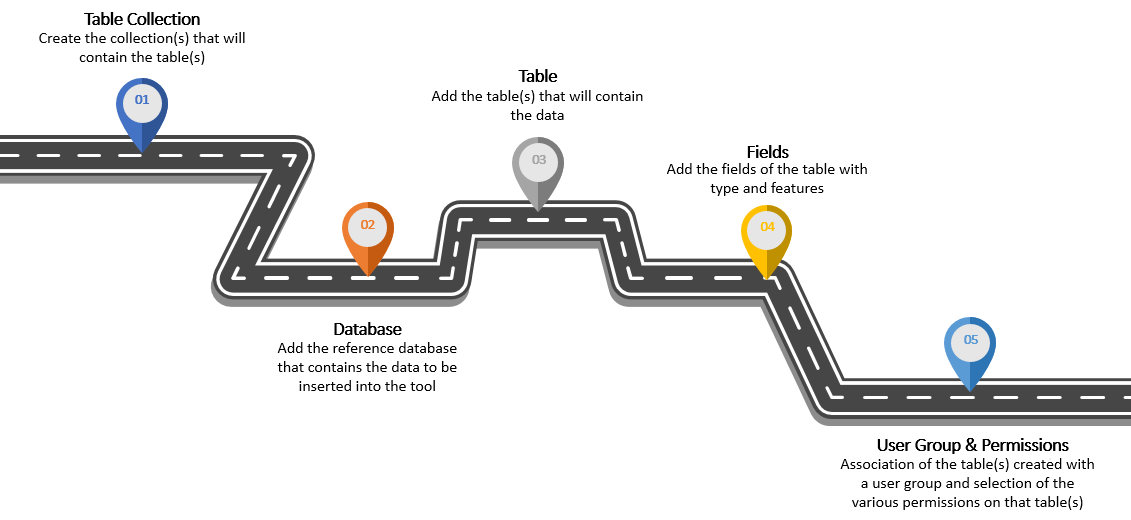
\includegraphics[width=15.8cm]{chapters/images/ch_3/BE_roadmap.png}
    \caption{Administrators' road-map.}
    \label{fig:BE_roadmap}
\end{figure}

From the road-map in Figure \ref{fig:BE_roadmap}, we can see that the workflow starts from the creation of table collections; this is done because it would be a good practice to have a collection in place when the tables are defined. After that, it is time to connect a database to the tool via the provided host, port, username and the password, which will be encrypted before storing in the Aurora instance. After a database connection test, to make sure that the provided connection parameters are correct, all necessary tables can be added, and whenever a new table is added, all fields that belong to the table are automatically added as well.

When the tables are in place, it is time to add users to the tool and assign them to user groups so that they have the appropriate permissions to operate on them.

\begin{figure}[!htb]
    \centering
    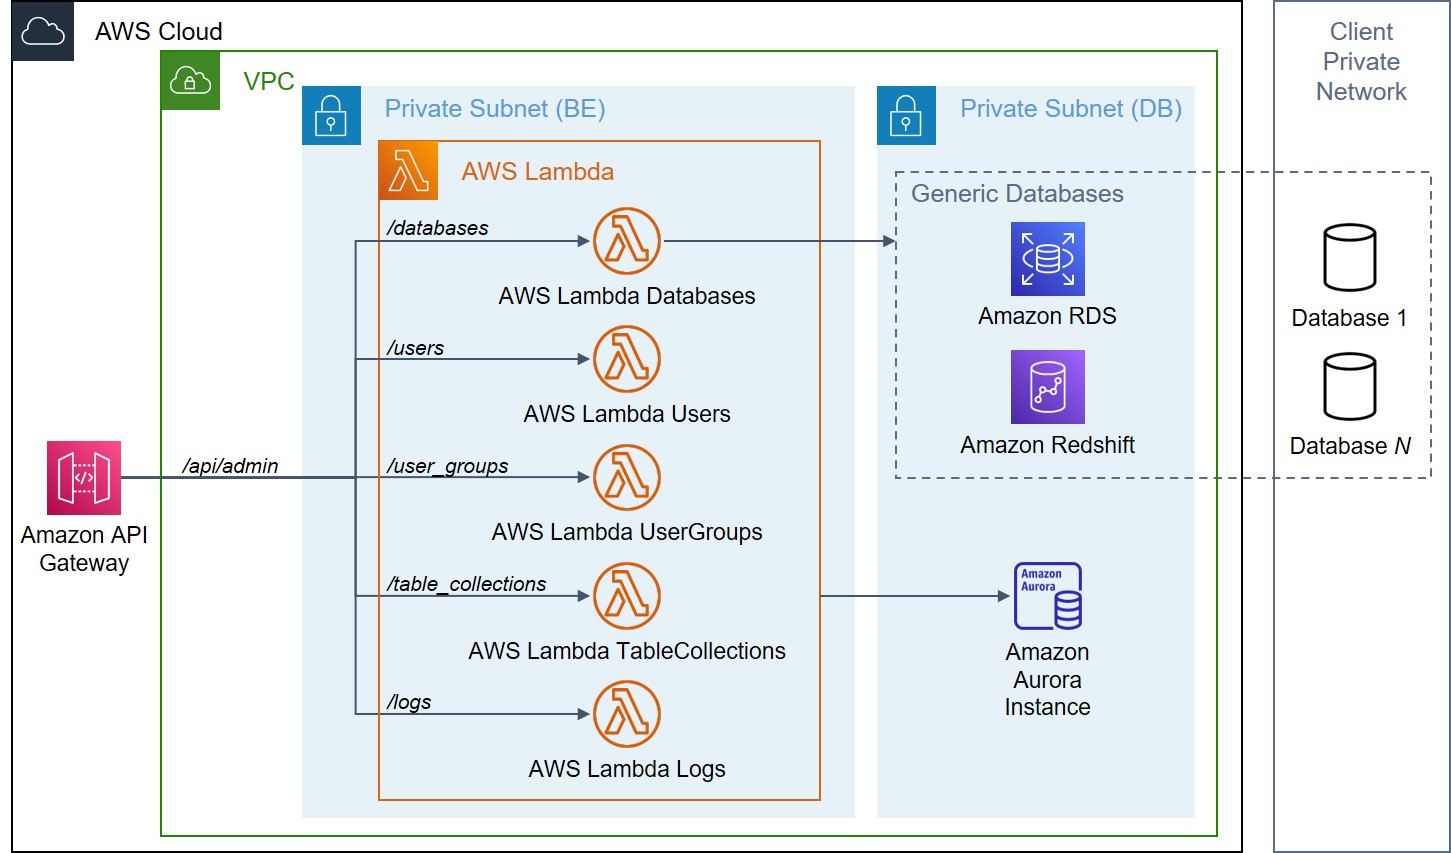
\includegraphics[width=15.8cm]{chapters/images/ch_3/BE_Admin.jpg}
    \caption{Administrators' side Back-End architecture.}
    \label{fig:BE_Admin}
\end{figure}



In Figure \ref{fig:BE_Admin} we can see the different functionalities for an administrator:
\begin{itemize}
    \item \code{/databases}: from this API an administrator can connect new databases to the tool, register new tables, and for each table register all fields; moreover, not all tables need to be manipulated by users; some of them can be added only to be referenced in other tables, as with foreign keys, to prevent integrity constraints problems.
    \item \code{/users}: this API is used to manage all users of the tool; keep in mind that the users of the tool are a subset of the users of the company.
    \item \code{/user\_groups}: from this API you can manage user groups, where all users and tables are associated with each other with different permission levels.
    \item \code{/table\_collections}: all table collections are maintained with this API. These collections are useful in the Front-End to display all tables from a drop-down menu, so that they are easily accessible by users.
    \item \code{/logs}: this API gives access to the logs of all operations performed on the registered tables by all users of the tool.
\end{itemize}

The full list of the APIs for the Administrators can be seen in Table \ref{tab:Admin_API_BE}.

\begin{table}[!htb]   
\small
  \centering
  \caption{List of APIs for the Administrator side.}
  \begin{tabular}{|l|p{4cm}|}
    \hline
    API List                                                             & Description                                                 \\\hline
    \code{/users}                                                        & Provide CRUD operations on the users of the tool            \\\hline
    \code{/user\_groups}                                                 & Manages all the user groups                                 \\\hline
    \code{/user\_groups/\{group\_id\}}                                   & Manage a given user group                                   \\\hline
    \code{/user\_groups/\{group\_id\}/tables}                            & View and manage the tables in a group                       \\\hline
    \code{/user\_groups/\{group\_id\}/users}                             & View and manage the users in a group                        \\\hline
    \code{/table\_collections}                                           & Manage all the collections                                  \\\hline
    \code{/table\_collections/\{table\_collection\_id\}}                 & View and manage the tables in a specific collection         \\\hline
    \code{/tables}                                                       & Returns all the tables                                      \\\hline
    \code{/databases}                                                    & To manage all the databases saved in the tool               \\\hline
    \code{/databases/\{database\_id\}/tables}                            & To manage the tables in a database                          \\\hline
    \code{/databases/\{database\_id\}/check\_connection}                 & Check if the connection to the database is working properly \\\hline
    \code{/databases/\{database\_id\}/tables/\{table\_id\}/fields}       & To manage the fields in a table                             \\\hline
    \code{/databases/\{database\_id\}/tables/\{table\_id\}/fields/order} & To change the order of the columns displayed to the user    \\\hline
    \code{/logs}                                                         & To view the logs of the operations in the tool              \\\hline
  \end{tabular}
  
  \label{tab:Admin_API_BE}
\end{table}

% \tikzstyle{every node}=[draw=black,thick,anchor=west]
% \tikzstyle{selected}=[draw=red,fill=red!30]
% \tikzstyle{optional}=[dashed,fill=gray!50]
% \begin{tikzpicture}[
%   grow via three points={one child at (0.5,-0.7) and
%   two children at (0.5,-0.7) and (0.5,-1.4)},
%   edge from parent path={(\tikzparentnode.south) |- (\tikzchildnode.west)}]
%   \node {\code{/admin}}
%     child { node {\code{/users}}}		
%     child { node {\code{/user\_groups}}
%         child {node {\code{/\{group\_id\}}}
%             child {node {\code{/tables}}}
%             child {node {\code{/users}}}
%         }
%     }
%     child [missing] {}
%     child [missing] {}
%     child [missing] {}
%     child { node {\code{/table\_collections}}
%          child {node {\code{/\{collection\_id\}}}}
%     }	
%     child [missing] {}
%     child { node {\code{/tables}}}
%     child { node {\code{/databases}}
%         child {node {\code{/\{database\_id\}}}
%             child {node {\code{/check\_connection}}}
%             child {node {\code{/tables}}
%                 child { node {\code{\{table\_id\}}}
%                         child {node {\code{/fields}}
%                             child {node {\code{/order}}}
%                         }
%                 }
%             }
%         }
%     }
%     child [missing] {}
%     child { node {\code{/logs}}}
%   ;
% \end{tikzpicture}



% %\pagebreak
\clearpage

\subsection*{User Side}
The user side of the Back-End contains all the logic of the possible manipulations they can perform on the actual tables distributed in the different databases. Note that no user can access tables for which s/he does not have permissions.  

In contrast to the administrator side, where the structure of the tool is static, meaning that each administrator will have the same graphical interface available, each user will have the interface adapted to their role in the tool. 
To be able to do it, it is necessary to provide the \emph{metadata} of the accessible tables to the Front-End, and checking on the Back-End side that each operations on the actual data is allowed. From a security perspective, this allows to thwart Man-in-the-Middle tampering.


\begin{figure}[!htb]
    \centering
    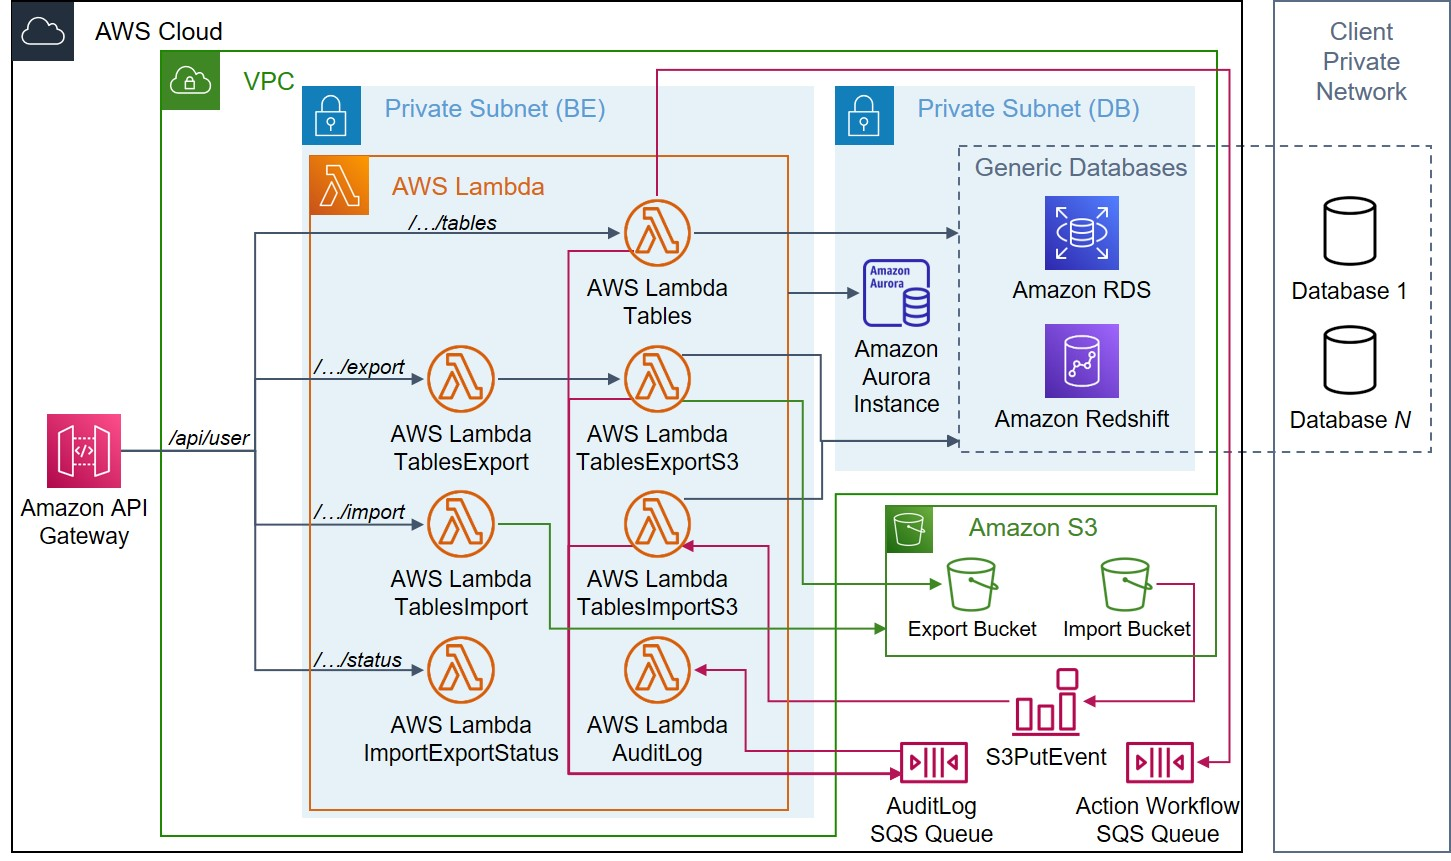
\includegraphics[width=15.8cm]{chapters/images/ch_3/BE_User.jpg}
    \caption{Users' side Back-End architecture.}
    \label{fig:BE_User}
\end{figure}

Figure \ref{fig:BE_User} represents the architecture behind the main users of the tool. After the successful execution of an allowed operation, that operation must be logged, and to do so, a message is sent via the SQS queue \emph{AuditLog} to another Lambda that will log it. The queue is used to decouple the operation execution to its logging so that the Lambda invoked by the user can return a response as quickly as possible to maintain some semblance of a real time feeling. The same reasoning is used also in the case of a table export, where no allowed operation is restricted during the export process, but not in case of import because there would be conflicts with any operations performed by the user, and for this reason no operation is allowed until the import process is completed.

Each API stems from the same base root, so each operation can refer the same table:
\begin{center}
    \begin{lstlisting}
        /table_collections/{collection_id}/tables/{table_id}
    \end{lstlisting}
\end{center}

% %\pagebreak

The most important endpoints accessible by the user are:
\begin{itemize}
    \item \code{/tables}: this API allows users to see and modify the content of all the tables they have permissions to. 
    \item \code{/export}: if the user is allowed to, with this API they can export the table in Excel format on their local machine. 
    \item \code{/import}: depending on the permissions given to the user, to update records, insert records or both, this API allows to load an Excel file to modify the table.
    \item \code{/status}: with this API it is possible to keep track of the import/export status.
\end{itemize}

Table \ref{tab:User_API_BE} shows the complete list of APIs for the User Side.
% \begin{tikzpicture}
%   [
%     grow                    = down,
%     sibling distance        = 6em,
%     level distance          = 10em,
%     edge from parent/.style = {draw, -latex},
%     every node/.style       = {font=\footnotesize},
%     sloped
%   ]
%   \node [root] {\code{/table\_collections/\{collection\_id\}/tables/\{table\_id\}}}
%     child { node [env] {metadata} edge from parent node [below] {} }
%     child { node [env] {records} edge from parent node [below] {} }
%     child { node [env] {export} edge from parent node [below] {} }
%     child { node [env] {import} edge from parent node [below] {} }
%     child { node [env] {} edge from parent node [below] {} }
%       ;
% \end{tikzpicture}



\begin{table}[!htb]   
\small
  \centering
  \caption{List of APIs for the User side.}
  \begin{tabular}{|l|p{6cm}|}
    \hline
    API List                                               & Description                                                                                                   \\\hline
    \code{/table\_collections}                             & Returns all collections with their own tables and user permissions                                            \\\hline
    \code{/.../metadata}                                   & Returns the metadata for a given table (e.g. table name, permissions, fields, ...)                            \\\hline
    \code{/.../records}                                    & Gives access to CRUD operations on data according to permissions                                              \\\hline
    \code{/.../}                                           & If available for a table, trigger the action execution                                                        \\\hline
    \code{/.../batchDelete}                                & If allowed, allows to delete multiple row in a table                                                          \\\hline
    \code{/.../export}                                     & If allowed, triggers the table export                                                                         \\\hline
    \code{/.../import}                                     & According to permissions, allow the import of an excel in \emph{INSERT}, \emph{UPDATE}, or \emph{UPSERT} mode \\\hline
    \code{/.../\{operation\_type\}/status}                 & Get the status of the current user's import and export operations on the table                                \\\hline
    \code{/.../\{operation\_type\}/status/\{request\_id\}} & Get the status of the given import/export operation                                                           \\
    \hline
  \end{tabular}
  
  \label{tab:User_API_BE}
\end{table}

\clearpage

\subsection{Front-End}
The APIs described in the Back-End section are not directly accessible by a user; they will interact with a Graphical User Interface to perform operations on the Data Entry Tool or the distributed databases. The Front-End section will use those API transparently to the user, while still showing some of them in the URI of the Tool website to make it clear to the user what resource it is trying to access. The complete list of APIs available to the users can be seen in Table \ref{tab:frontEndAPIs}.

\begin{table}[!htb]   
\small
  \centering
  \caption{APIs exposed by the Front-End.}
  \begin{tabular}{|l|p{3.5cm}|}
    \hline
    API List                                                           & Description                                                                     \\\hline
    \code{/user}                                                       & User's dashboard and main page                                                  \\\hline
    \code{/user/table\_collections/:tableCollectionId/tables/:tableId} & Gives access to view and manipulate the given table                             \\\hline
    \code{/admin/databases}                                            & To manage the databases                                                         \\\hline
    \code{/admin/databases/:dbId/tables}                               & To manage the tables in a given database                                        \\\hline
    \code{/admin/databases/:dbId/tables/:tableID/fields}               & to manage the fields in a given table                                           \\\hline
    \code{/admin/users}                                                & To manage the users of the Tool                                                 \\\hline
    \code{/admin/user-groups}                                          & To create the association between users and tables and granting the permissions \\\hline
    \code{/admin/table-collections}                                    & To manage all the table collections                                             \\\hline
    \code{/admin/logs}                                                 & To view logs of operations performed by users                                   \\\hline
  \end{tabular}
  
  \label{tab:frontEndAPIs}
\end{table}


\begin{figure}[!htb]
    \centering
    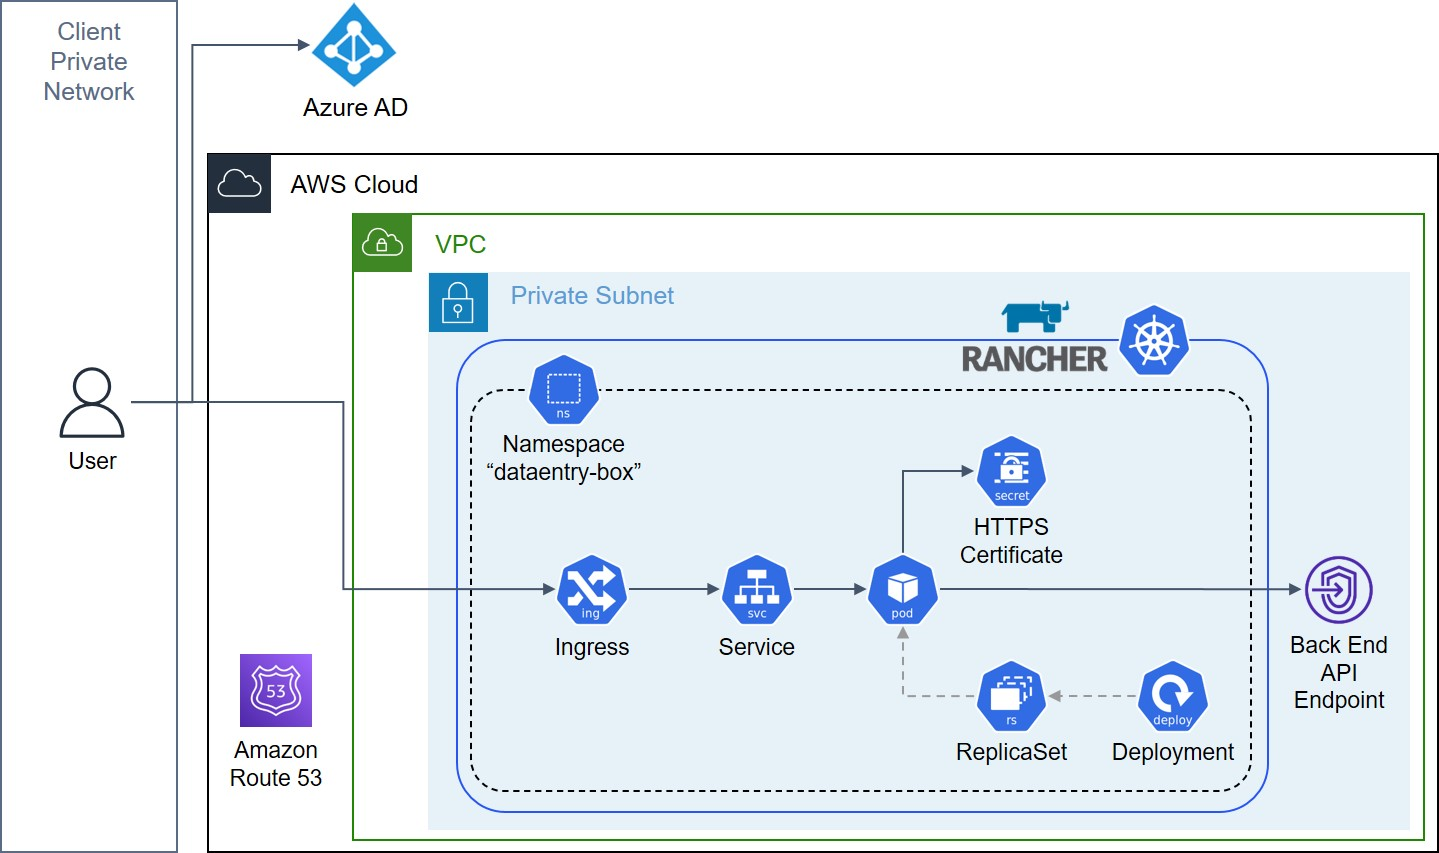
\includegraphics[width=15.8cm]{chapters/images/ch_3/FE.jpg}
    \caption{Front-End architecture.}
    \label{fig:FE}
\end{figure}
As shown in Figure \ref{fig:FE}, the Front-End application consists of a Docker container that is hosted on an instance of Rancher, which exposes a URL to access the Tool that is accessible only from the corporate intranet.

\subsubsection{Web Application Container}
The aforementioned container is based on an NGINX \cite{nginx} image, an open source software which has capabilities as web server and reverse proxy. The web server, listening on port 80, is used to serve the Tool's end users the Front-End of the application, while the reverse proxy capability is used to redirect user requests to the appropriate Back-End server, in this case to the proper Back-End API.


\subsubsection{Web Application Instance}
To create an instance of the Front-End container image, which is called a \emph{Pod} in Rancher, other than the image itself, it is necessary to provide an entry point to the Tool. This is done via the \code{Ingress} service: through it, the NGINX web server URL and listening port are bound to the Ingress service URL and listening port. Moreover, it is provided a TLS certificate to ensure security and encryption to the data exchanged between the user and the application.


% spiegare come è istanziato il container su k8s





\subsection*{Authentication \& Authorization}
As described before, in order to access the Tool a user has to provide his/her own username to the company's Azure Active Directory which will issue a token that will be verified via the Lambda Authorizer seen in the previous section. If the user is not present in the Aurora database, or if s/he is present but does not have access to any table yet, the pages represented in Figure \ref{fig:403Empty} will be shown.


\begin{figure}[!htb]
  \begin{subfigure}{\linewidth}
    \centering
    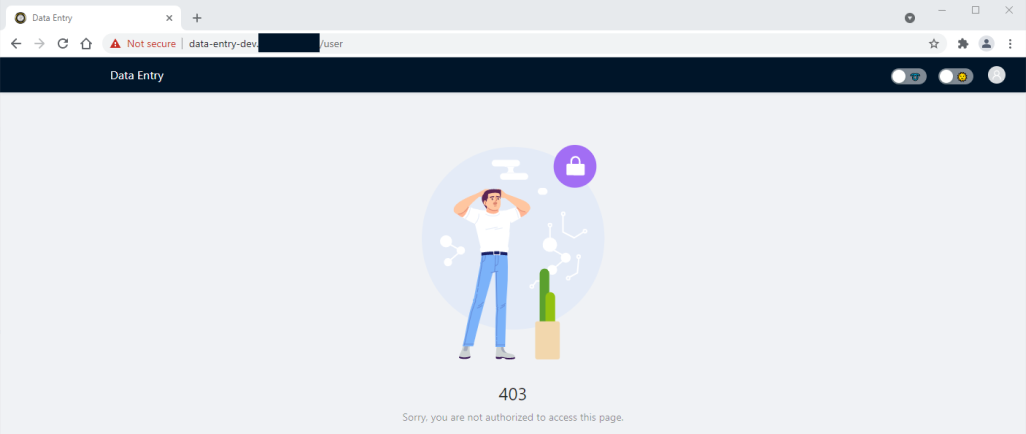
\includegraphics[width=15.8cm]{chapters/images/ch_3/FE/403.png}
    \caption{Unauthorized access.}
  \end{subfigure}\par\medskip
  \begin{subfigure}{\linewidth}
    \centering
    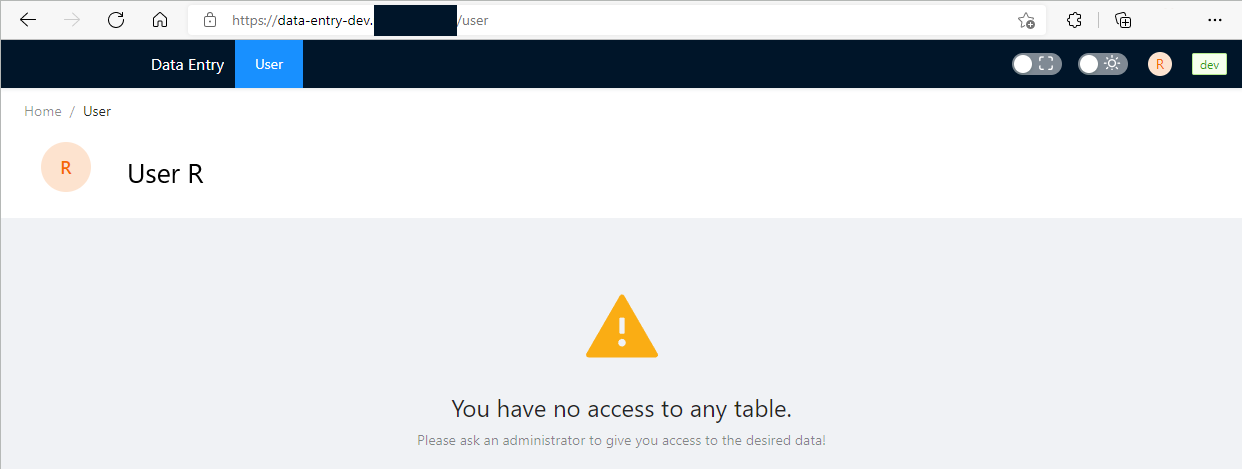
\includegraphics[width=15.8cm]{chapters/images/ch_3/FE/empty.png}
    \caption{No table available.}
  \end{subfigure}\par\medskip
  \caption{Restricted access pages.}
  \label{fig:403Empty}
\end{figure}
 

\subsection*{Common Features} 
All the tables, shown in the figures that will follow, have some basic operations in common that are performed on the Back-End side to avoid overloading the client and because it is easier to perform while retrieving the data from the different databases. 

\subsubsection{Pagination}
All the tables have the option to be paginated, which means changing the number of rows displayed to the user; this is done by adding the optional query parameters \code{page} and \code{pageSize} to the request to the Back-End. 
These two parameters represent, respectively, the page number and the number of rows to be displayed in the table, and they are used in the process of data retrieval to set the amount of rows to be fetched and with which offset to take them, as shown in the Code Sample \ref{code:pagination}. 

\begin{lstlisting}[
    language=SQL, 
    caption={SQL representation of the pagination process.}, 
    label={code:pagination},
    captionpos=b
]
SELECT ...
FROM table
LIMIT pageSize OFFSET page
\end{lstlisting}

\subsubsection{Filtering}
Whenever a magnifying glass icon is displayed next to a column name, it means that you can filter the table based on a value provided for that column. Also, if the columns allow it, it is possible to apply a filter on more than one column at a time, because the filtering process is additive. This is possible thanks to the query parameter \code{filters} which contains an array of filters to apply to the table; a filter is composed of: 
\begin{itemize}
    \item an operation on how to filter the rows, like \emph{equality} to get the rows with the same value as the provided one, \emph{greater than} to get all the elements which are greater than the provided one. The full list of operations is available in Table \ref{tab:filtering} and the representation of those filters can be seen in Figure \ref{fig:filtering};
    \item the name of the column to filter for;
    \item the value for which to filter; this could be a single value, a couple of values, and a list of values.
\end{itemize}
 As shown in the Code Sample \ref{code:filtering}, the filtering process is translated into a set of \emph{WHERE} conditions, and since the filtering process is additive, each condition is linked with a \emph{AND} statement.

\begin{lstlisting}[
    language=SQL, 
    caption={SQL representation of the filtering process.}, 
    label={code:filtering},
    captionpos=b
]
SELECT ...
FROM table
WHERE columnName1 = toCompare1 AND columnName2 > toCompare2 AND ...
\end{lstlisting}

\begin{figure}[!htb]

  \begin{subfigure}{\linewidth}
    \centering
    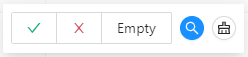
\includegraphics[width=.3\linewidth]{chapters/images/ch_3/FE/Common/boolean.png}
    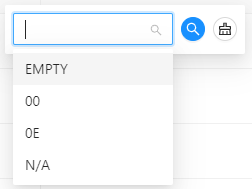
\includegraphics[width=.3\linewidth]{chapters/images/ch_3/FE/Common/list.png}
    \caption{Filter by a boolean value or from a list of possible values.}
  \end{subfigure}\par\medskip
  \begin{subfigure}{\linewidth}
    \centering
    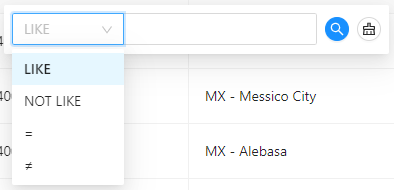
\includegraphics[width=.3\linewidth]{chapters/images/ch_3/FE/Common/string.png}
    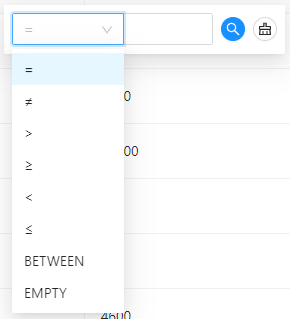
\includegraphics[width=.3\linewidth]{chapters/images/ch_3/FE/Common/numeric.png}
    \caption{Filter by a given alphanumeric word or a number.}
  \end{subfigure}\par\medskip
  \begin{subfigure}{\linewidth}
    \centering
    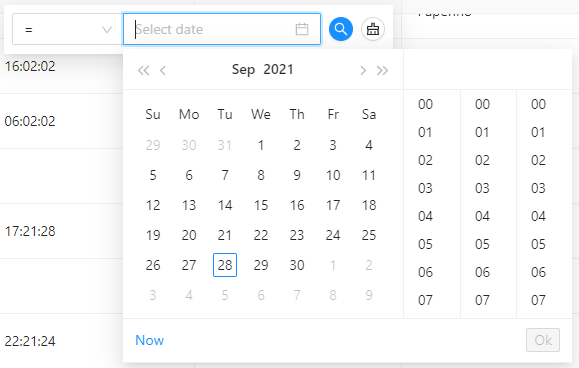
\includegraphics[width=.3\linewidth]{chapters/images/ch_3/FE/Common/date_time.png}
    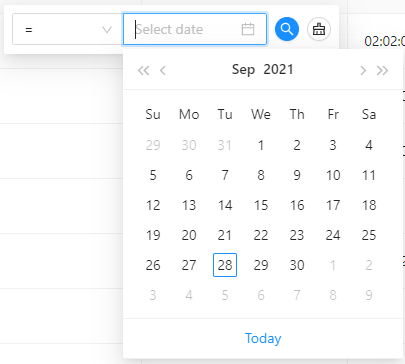
\includegraphics[width=.3\linewidth]{chapters/images/ch_3/FE/Common/date.png}
    \caption{Filter by a date and a given time or just the date.}
  \end{subfigure}
  \caption{Different filtering options based on column type.}
  \label{fig:filtering}
\end{figure}


\begin{table}[!htb]   
\small
  \centering
  \caption{List of the available operations.}
  \begin{tabular}{|l|p{9cm}|}\hline
    Operation    & Description                                                                         \\\hline
    EQ           & Takes the values that are equal to the provided one                                 \\\hline
    NOT\_EQ      & Takes only the values that are \textbf{not} equal to the input                      \\\hline
    GT           & Tkes the values that are greater than the input                                     \\\hline
    GTQ          & Takes the values that are greater or equal than the input                           \\\hline
    LT           & Takes the values that are less than the input                                       \\\hline
    LTQ          & Takes the values that are less or equal than the input                              \\\hline
    IN           & Takes the values that are present in the provided list                              \\\hline
    NOT\_IN      & Takes the values that are \textbf{not} present in the provided list                 \\\hline
    LIKE         & Takes the values that are similar to the provided one (case sensitive)              \\\hline
    NOT\_LIKE    & Takes the values that are \textbf{not} similar to the provided one (case sensitive) \\\hline
    I\_LIKE      & Takes the values that are similar to the provided one (case insensitive)            \\\hline
    BETWEEN      & Takes the values that are in between the provided input couple                      \\\hline
    NOT\_BETWEEN & Takes the values that are \textbf{not} in between the provided input couple         \\\hline
    IS\_NULL     & Takes the values that are null                                                      \\\hline
  \end{tabular}
  
  \label{tab:filtering}
\end{table}

\subsubsection{Sorting}
Lastly, if the up and down arrows are present next to the column name, it is possible to sort the rows of the table by the values in that column, either in ascending or descending order; also, just like the filtering operation, the sorting operation is additive, meaning that it is possible to sort a table by multiple columns. Like the previous operations, this one also uses a query parameters, \code{orderBy}, that contains a list of columns to order by and which order to use for each column. To make it easier for the user to figure out which columns they applied the sort to, if it was applied to more than one, a number appears next to the column name, as shown in Figure \ref{fig:sorting}.

\begin{figure}[!htb]
    \centering
    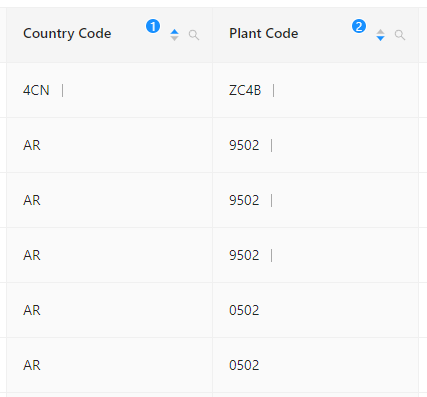
\includegraphics[width=9cm]{chapters/images/ch_3/FE/Common/sorting.png}
    \caption{Sort order for multiple columns.}
    \label{fig:sorting}
\end{figure}

\subsubsection{Actions on records}
The previous ones were operations that affected the entire table, while the following ones are actions that interest the single rows of a table. As shown in Figure \ref{fig:actions}, there are 5 possible actions that can be performed on the records:
\begin{itemize}
    \item  \emph{New Record}:  this button allows the insertion of a new record in the table by opening a menu on the right of the table to enter the specific values.
    \item  \emph{Edit}: this button opens the same menu as ``\emph{New Record}'', but filled with the values of the selected record; from here it is possible to change the values according to the necessary update;
    \item  \emph{Delete}: this operation deletes the record. Since it can be a dangerous operation, before deleting a row a confirmation pop up appears asking if you want to proceed. It is also possible to enable a table for the deletion of multiple rows.
    \item  \emph{Duplicate}: duplicates the current record. This feature helps a user not to have to retype all the values for a new record if most of them are the same as for another one;
    \item \emph{Refresh}: with this button the table can be refreshed at any moment to visualize any new values.
\end{itemize}

\begin{figure}[!htb]
    \centering
    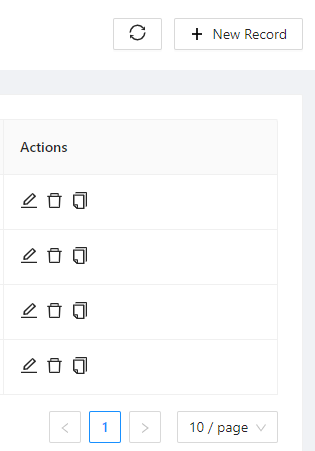
\includegraphics[width=7cm]{chapters/images/ch_3/FE/Common/actions.png}
    \caption{Actions allowed on records.}
    \label{fig:actions}
\end{figure}

Keep in mind that all of these actions and operations are always enabled for the Administrator side, while for the User side, excluding pagination and refresh, they must be enabled by granting permission to the user group that will access the particular table.

\clearpage

\subsection*{Administrator Side}
If the user is present in the database and is recognized to be also an administrator, s/he will be redirected to the first page of the Administrator Side, the \emph{Databases} page, shown in Figure \ref{fig:adminHome}, where s/he will see all the databases already registered to be managed by the Tool. 

\subsubsection{Databases}
From this page an administrator can add new databases and manage the existing ones. In addition to the basic operations established above, for each database it is also possible to check at any time that the connection to it is working. 

\begin{figure}[!htb]
    \centering
    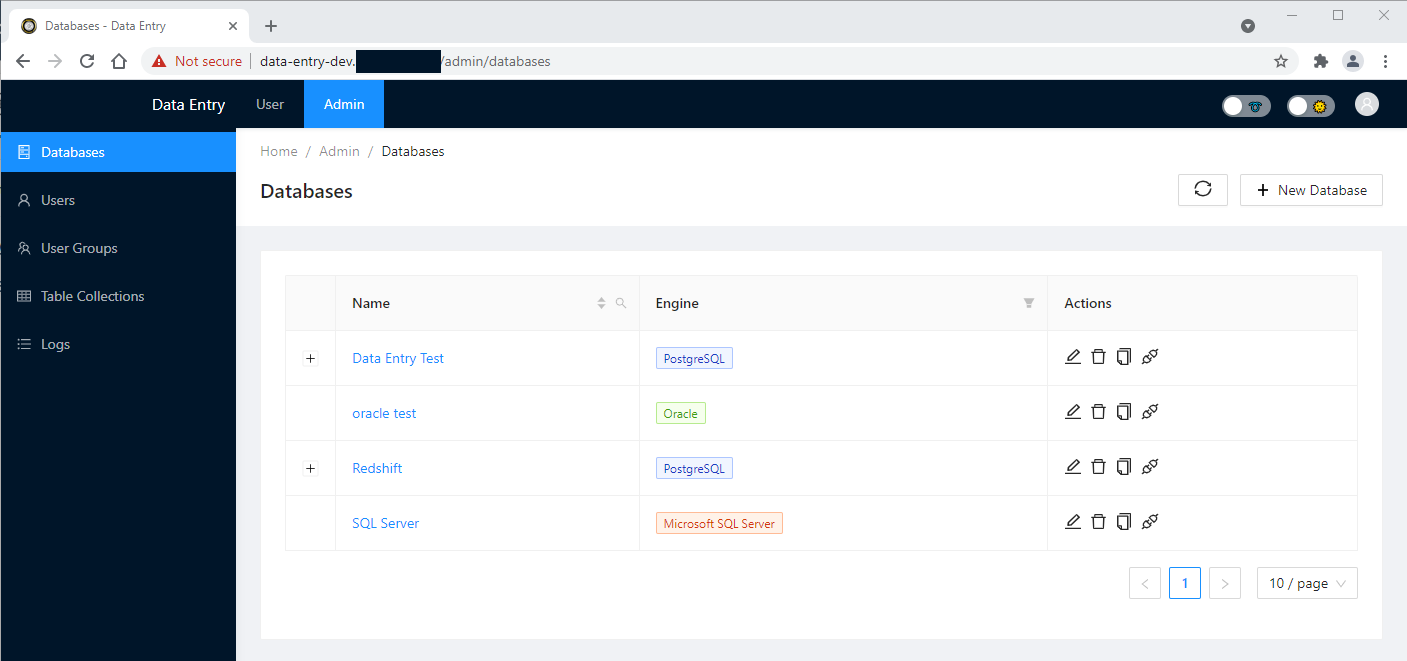
\includegraphics[width=15.8cm]{chapters/images/ch_3/FE/Admin/admin_section.png}
    \caption{Administrator's homepage.}
    \label{fig:adminHome}
\end{figure}

The information required to add, or edit, a database, as shown in the Figure \ref{fig:editDB}, is:
\begin{itemize}
    \item \emph{Database Name}: this is the name that is going to be displayed in the Tool;
    \item \emph{Engine}: the Database Management System that powers the database; the available options are \textbf{PostgresSQL}, \textbf{OracleDB}, and \textbf{Microsoft SQL Server};
    \item \emph{Hostname \& Port}: this is the connection string to the database with the relative port;
    \item \emph{Instance Name}: this is the actual name of the database on its hosting machine;
    \item \emph{Database User \& Password}: these are the credentials used to access the database; all tables that are intended to be used by the Tool must be accessible to this user.
\end{itemize}

\begin{figure}[!htb]
    \centering
    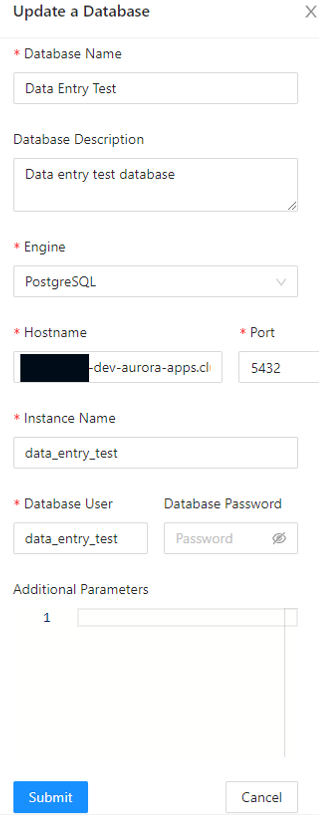
\includegraphics[width=7cm]{chapters/images/ch_3/FE/Admin/editDB.png}
    \caption{Add/edit form for a database.}
    \label{fig:editDB}
\end{figure}

\subsubsection{Tables}
Once a database has been added, it is time to add to the Tool the tables that will be used by the users. To do this, we need to enter the database we have just created, where we will see the page in Figure \ref{fig:tables}. From here it is possible to add or edit any table to which, as mentioned before, the user of the database used for the connection has access.
\begin{figure}[!htb]
    \centering
    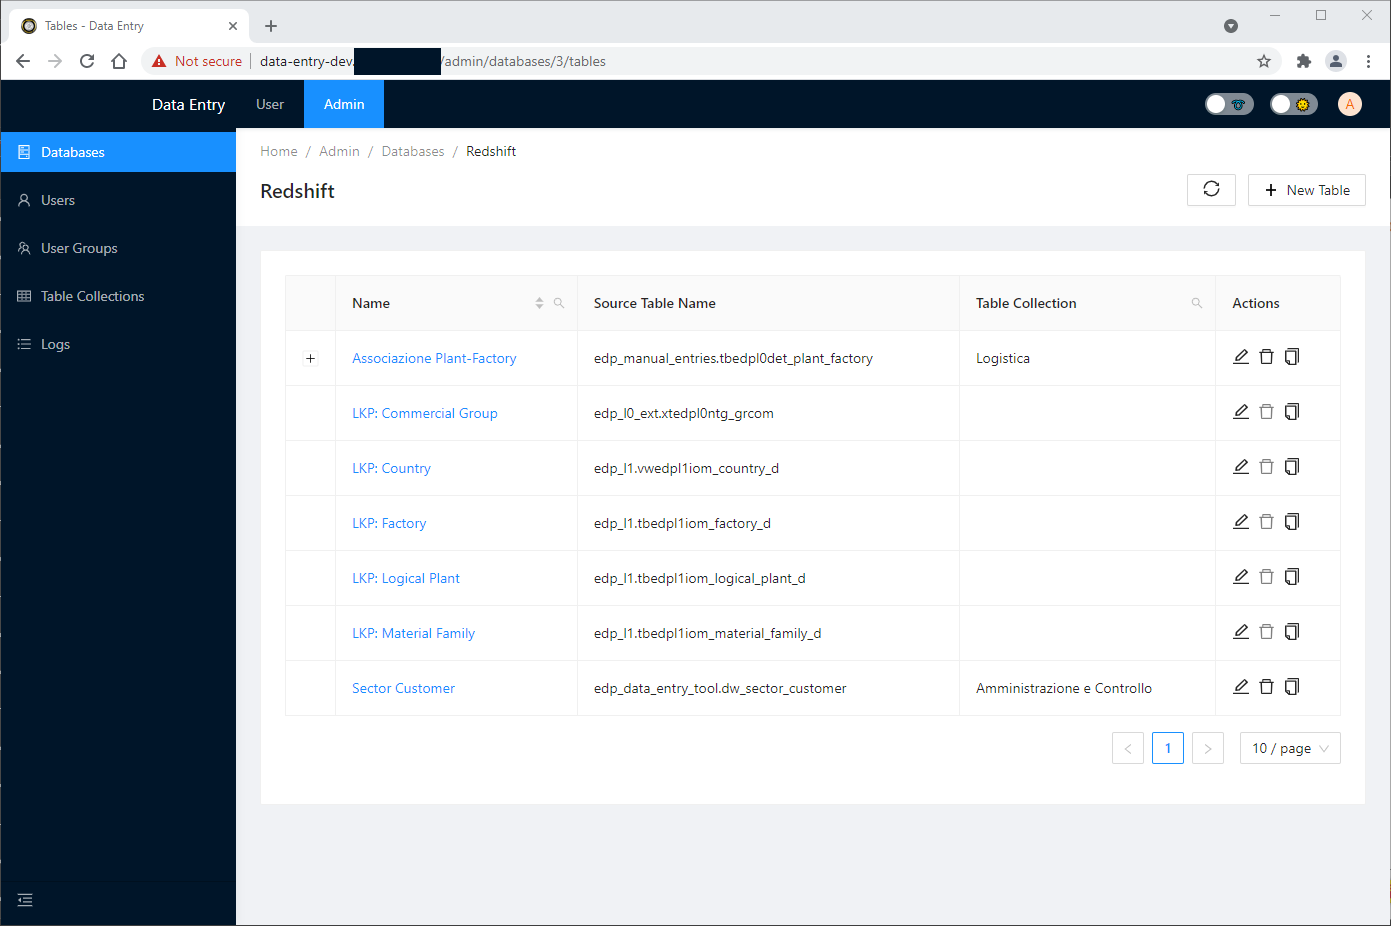
\includegraphics[width=15.8cm]{chapters/images/ch_3/FE/Admin/tables.png}
    \caption{Tables management page.}
    \label{fig:tables}
\end{figure}

Figure \ref{fig:editTab} shows the minimum information needed to add or edit a table:
\begin{itemize}
    \item \emph{Table Name}: the name that will be displayed in the Tool;
    \item \emph{Source Schema Name}: the schema associated to the table;
    \item \emph{Source Table Name}: original name of the table in the database
\end{itemize}

\begin{figure}[!htb]
    \centering
    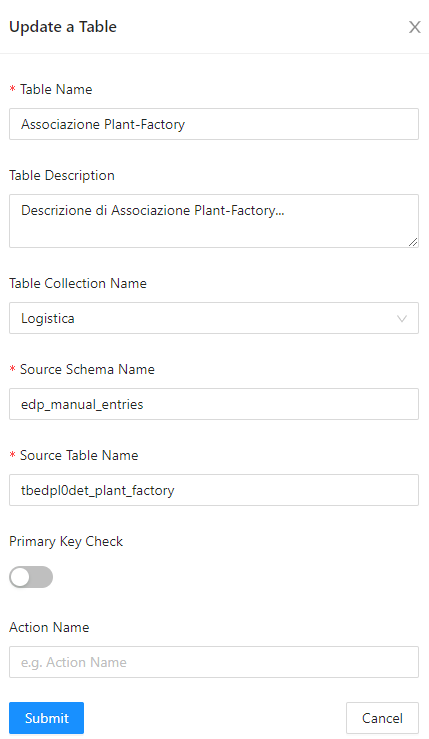
\includegraphics[width=8cm]{chapters/images/ch_3/FE/Admin/editTable.png}
    \caption{Add/edit form for a table.}
    \label{fig:editTab}
\end{figure}

The original schema and table name are used to retrieve information about the table, in this case, as we will see in the next section, the columns that make it up.
As for deleting tables, not all of them can be deleted at will, because they can be used by others as lookup tables from which to retrieve data, much like foreign keys.



\subsubsection{Fields}
When a table is added, all fields associated to it are automatically added to the Tool, and by looking at the breadcrumbs at the top of the page, it is possible to see to which table the fields shown in Figure \ref{fig:fields} belong. 
\begin{figure}[!htb]
    \centering
    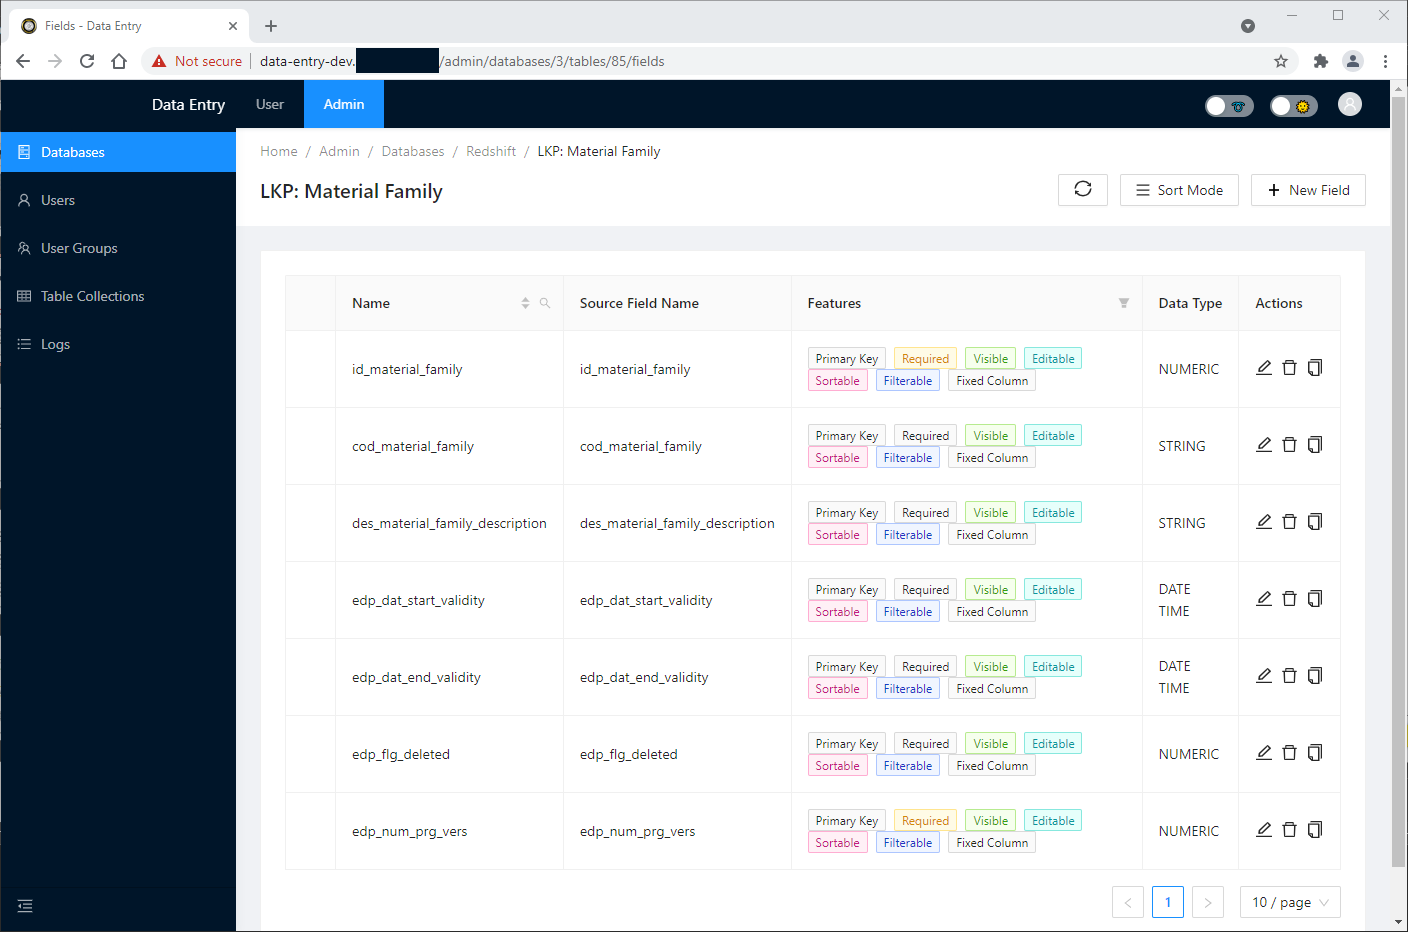
\includegraphics[width=15.8cm]{chapters/images/ch_3/FE/Admin/fields.png}
    \caption{Fields management page.}
    \label{fig:fields}
\end{figure}

During the field retrieval process, the column datatype is parsed and associated with the field in the Tool; this datatype is important because the filtering and sorting operations and data entry constraints depend on it. For example, a \emph{Numeric} field may have constraints such as a minimum or maximum value, or floating-point precision, and can be ordered by increasing value. This information is retrieved during the table insertion, if available, otherwise it needs to be added by hand in the form shown in Figure \ref{fig:editFie}. Here the bare minimum information needed to edit a filed is:
\begin{itemize}
    \item \emph{Field Name}: the name that will be displayed in the Tool. It defaults to be the same as the Source Field Name;
    \item \emph{Source Field Name}: original name of the column in the table;
    \item \emph{Data Type}: the datatype of the column. Note that different datatype may have more required information, as shown in Figure \ref{fig:types}
\end{itemize}

\begin{figure}[!htb]

  \begin{subfigure}{\linewidth}
    \centering
    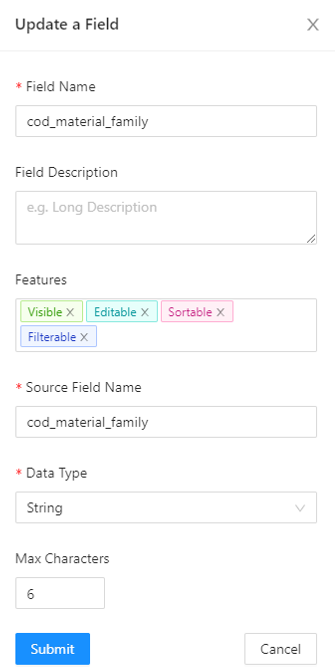
\includegraphics[width=7cm]{chapters/images/ch_3/FE/Admin/editField.png}
    \caption{Edit form for a field.}
    \label{fig:editFie}
  \end{subfigure}
  \begin{subfigure}{\linewidth}
    \centering
    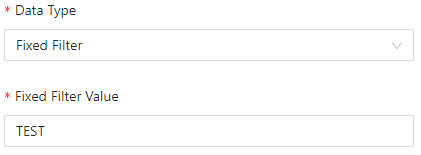
\includegraphics[width=5cm]{chapters/images/ch_3/FE/Admin/fixed_filter.png}
    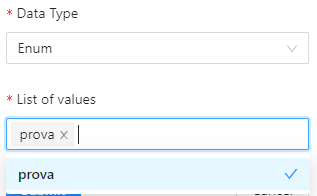
\includegraphics[width=5cm]{chapters/images/ch_3/FE/Admin/enum.png}
    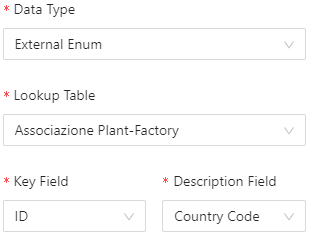
\includegraphics[width=5cm]{chapters/images/ch_3/FE/Admin/external_enum.png}
    \caption{Different constraints for the datatype.}
    \label{fig:types}
  \end{subfigure}
  \caption{Field management form.}
  \label{editFields}
\end{figure}


\subsubsection{Users}

The next item in the left-hand menu is the \emph{Users} page, displayed in Figure \ref{fig:users}. From this page an administrator can add a user to the database, which means granting access to the Tool, provided that this user is present in the client's Azure Active Directory. From here you can grant or revoke a user's administrator status, however an administrator cannot revoke his/her own status.
\begin{figure}[!htb]
    \centering
    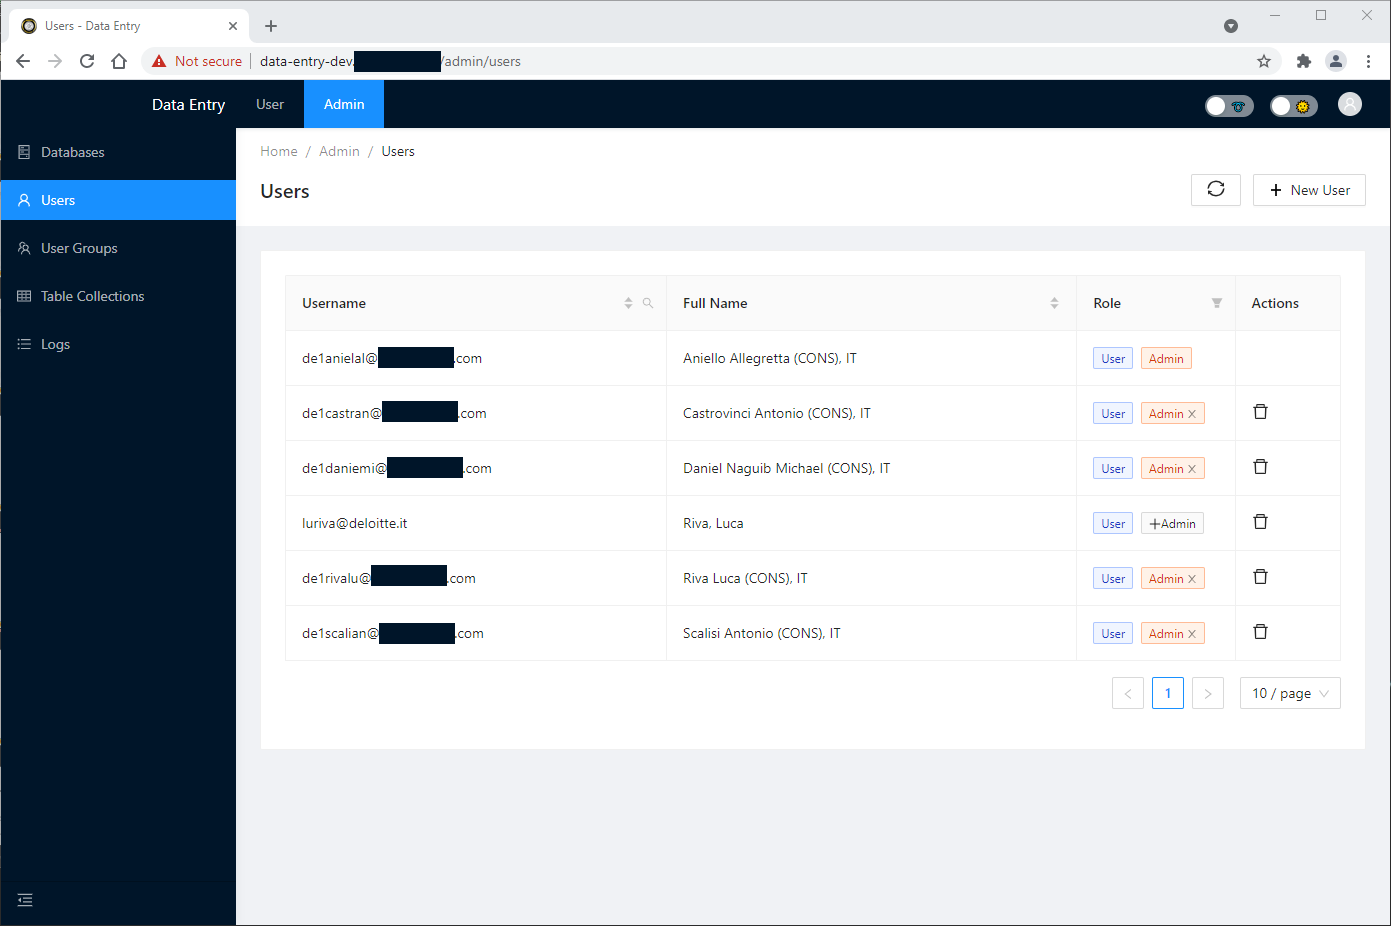
\includegraphics[width=15.8cm]{chapters/images/ch_3/FE/Admin/users.png}
    \caption{Users management page.}
    \label{fig:users}
\end{figure}

\subsubsection{User Groups}
Moving forward in the menu there is the \emph{User Groups} page, shown in Figure \ref{fig:userGroup}. Here all users are associated with tables and have different permissions based on the group. As we can see, there is a counter of how many users and tables each group has. Also, as described above in the Database section, the same user can be associated with different groups, and the same goes for tables; this means that the permission level on the same table can vary between groups, and if the user belongs to different groups where the same table exists, the permission level on that particular table would be the sum of the permissions of each group.

\begin{figure}[!htb]
    \centering
    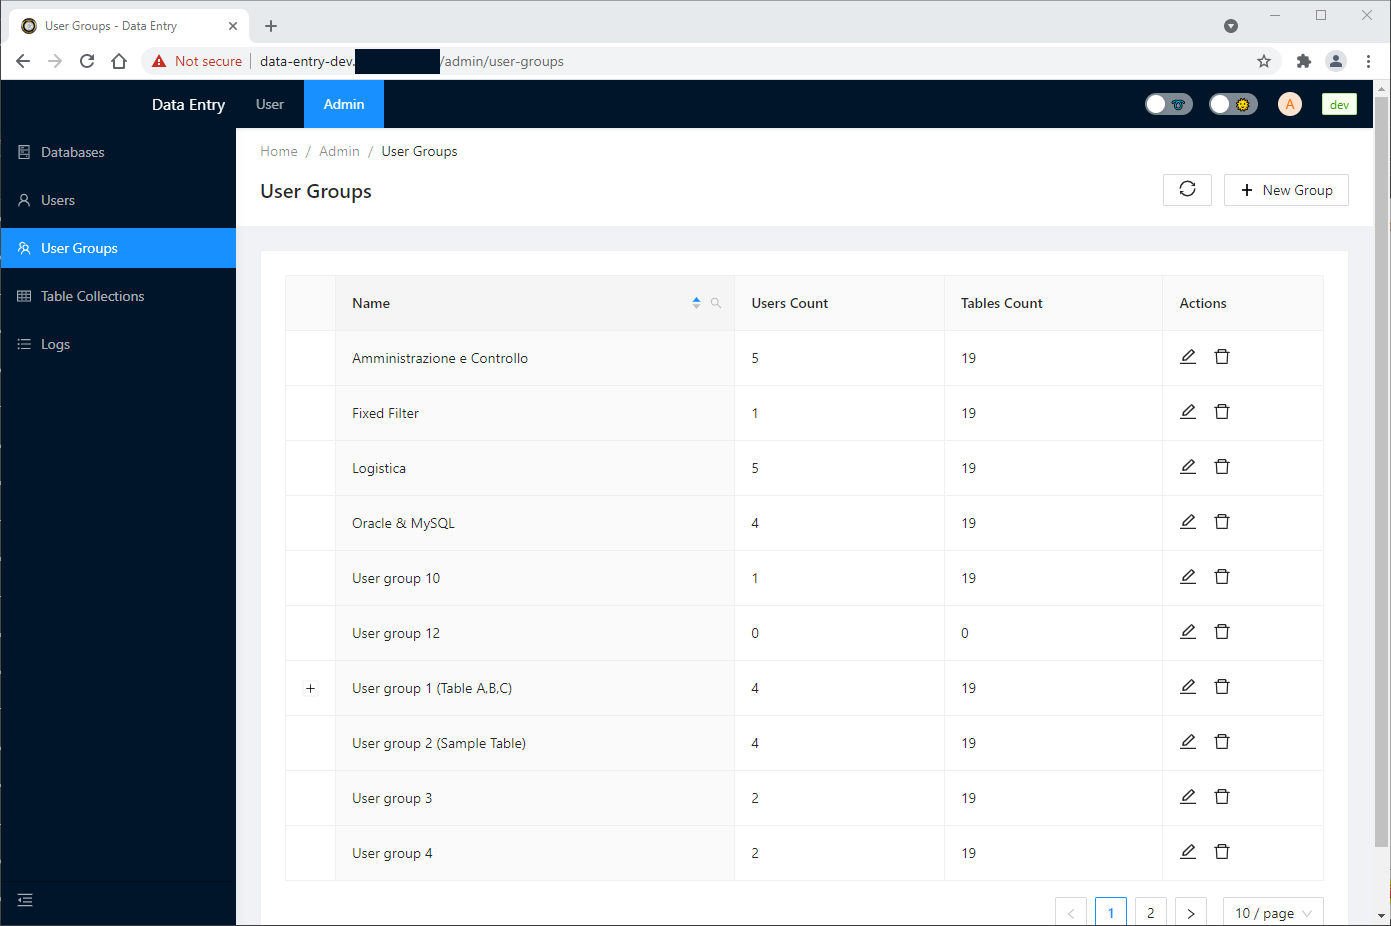
\includegraphics[width=15.8cm]{chapters/images/ch_3/FE/Admin/user_group.png}
    \caption{User groups management page.}
    \label{fig:userGroup}
\end{figure}

Figure \ref{a} shows the form used to make associations in a group, i.e. users and tables, other than the name of the group, while Figure \ref{b} shows the permissions that can be given the users accessing a table.

\begin{figure}[!htb]
  \centering
  \begin{subfigure}{\linewidth}
    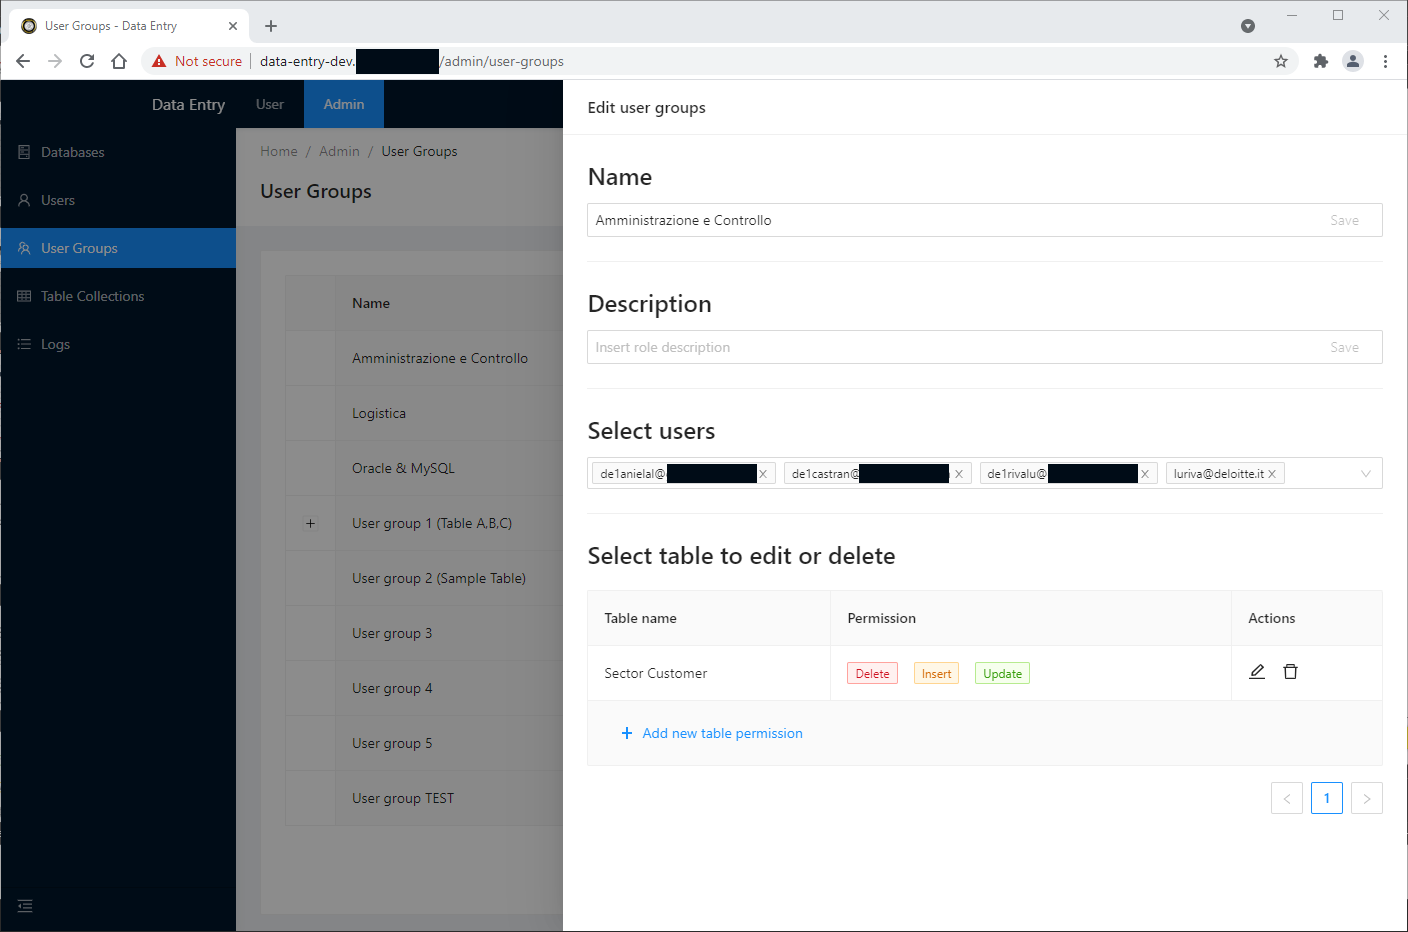
\includegraphics[width=15.8cm]{chapters/images/ch_3/FE/Admin/edit_user_group.png}
    \caption{Add/edit form for a user group.}
    \label{a}
  \end{subfigure}
  \begin{subfigure}{\linewidth}
    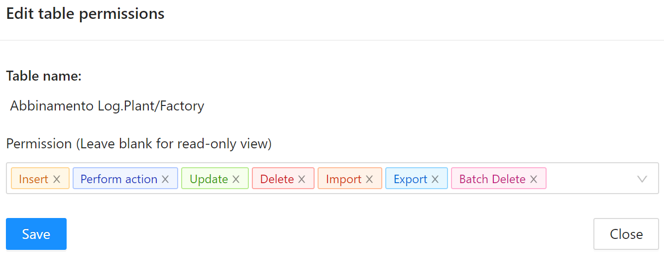
\includegraphics[width=15.8cm]{chapters/images/ch_3/FE/Admin/tabPermissions.png}
    \caption{Permissions level form.}
    \label{b}
  \end{subfigure}
  \caption{Group management form.}
  \label{fig:editGroup}
\end{figure}


\subsubsection{Table Collections}
Figure \ref{fig:collect} shows the next entry in the menu, the \emph{Table Collections} page. The collections managed here are used to group the tables, thus making their use well organized for the user.
\begin{figure}[!htb]
    \centering
    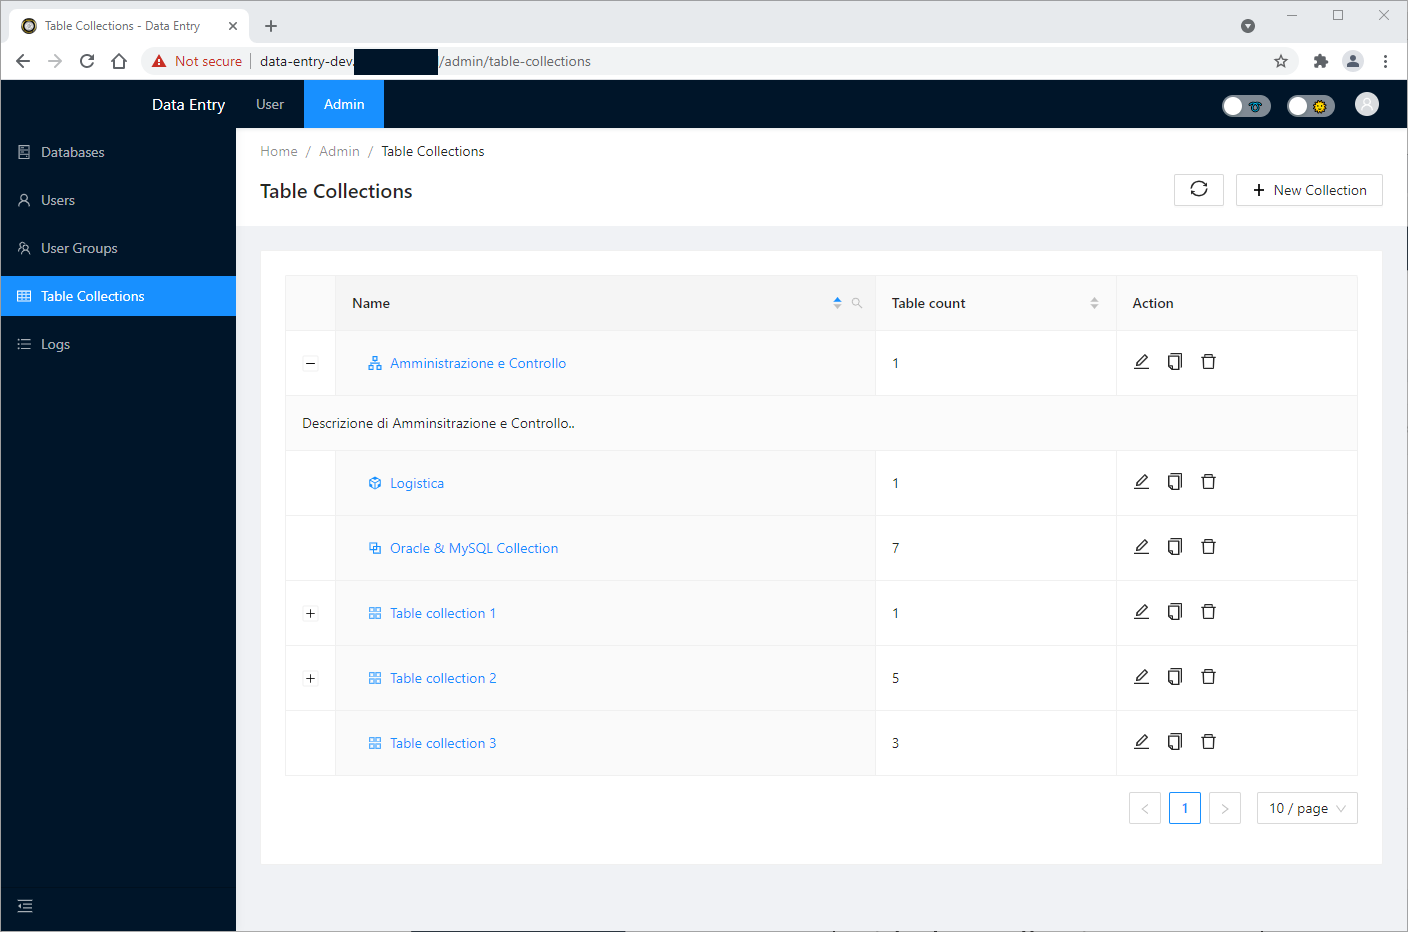
\includegraphics[width=15.8cm]{chapters/images/ch_3/FE/Admin/table_collections.png}
    \caption{Table collections management page.}
    \label{fig:collect}
\end{figure}

In addition to the name, as shown in Figure \ref{fig:editCollect}, a collection is characterized by an icon; this icon is used to identify the collection when the left menu is minimized to give more room to the table.

\begin{figure}[!htb]
    \centering
    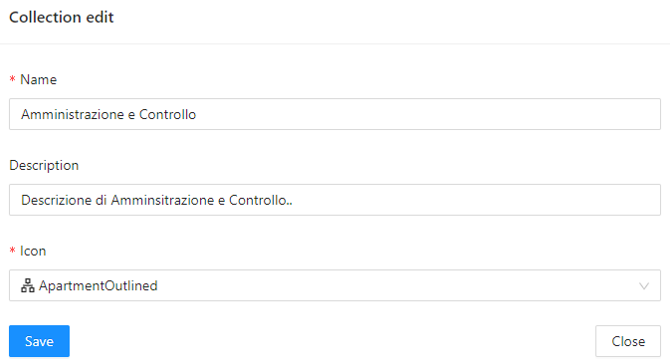
\includegraphics[width=11cm]{chapters/images/ch_3/FE/Admin/editCollect.png}
    \caption{Add/edit form for a collection.}
    \label{fig:editCollect}
\end{figure}

\subsubsection{Logs}
The last entry in the menu for the Administrator side is the \emph{Logs} page, here represented by Figure \ref{fig:logs}. This page is used to observe all the operations performed by the users of the Tool and the result of each of them.
\begin{figure}[!htb]
    \centering
    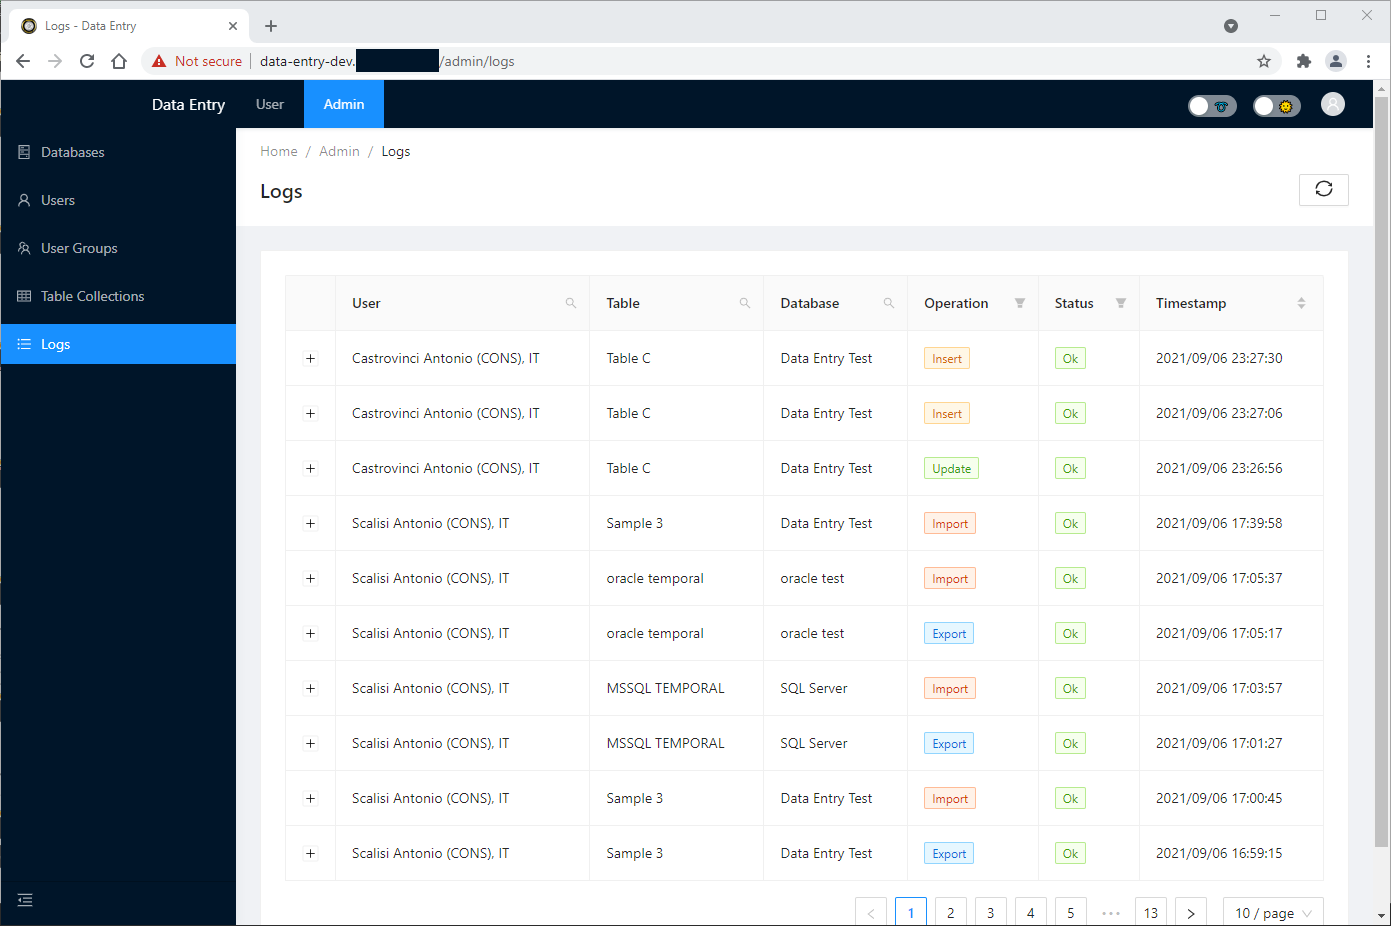
\includegraphics[width=15.8cm]{chapters/images/ch_3/FE/Admin/logs.png}
    \caption{Logs page.}
    \label{fig:logs}
\end{figure}

In case of a failed operation, it is possible to observe the error returned from the Tool, here in Figure \ref{fig:err}, and the input that caused it.

\begin{figure}[!htb]
    \centering
    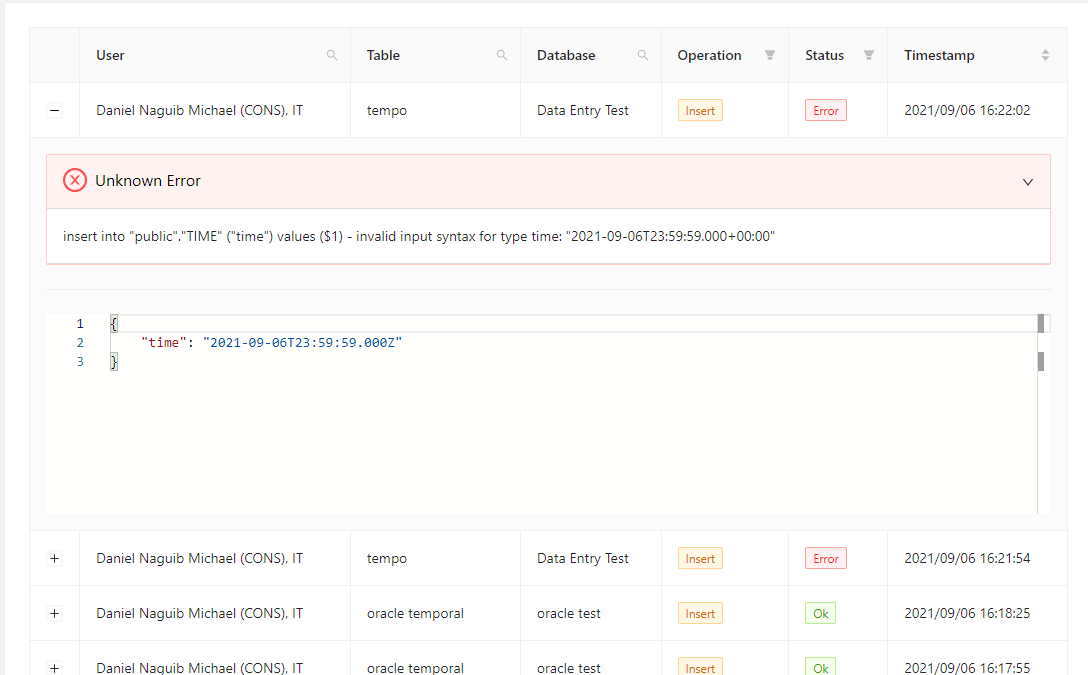
\includegraphics[width=15.8cm]{chapters/images/ch_3/FE/Admin/error.png}
    \caption{Failed operation with the associated error.}
    \label{fig:err}
\end{figure}

%\pagebreak
\clearpage
\subsection*{User Side}
As anticipated in the Back-End section, the User Side of the Front-End is very dynamic due to the fact that each user can access different tables. This is very evident from the homepage that welcomes the users of the Tool shown in Figure \ref{fig:home}. As we can see, users will see a series of cards representing the different table collections they have access to. Within each card, all accessible tables are listed with an overview of the permissions enabled for each. Note also that the same collections are visible and easily accessible in the menu on the left. 

\begin{figure}[!htb]
    \centering
    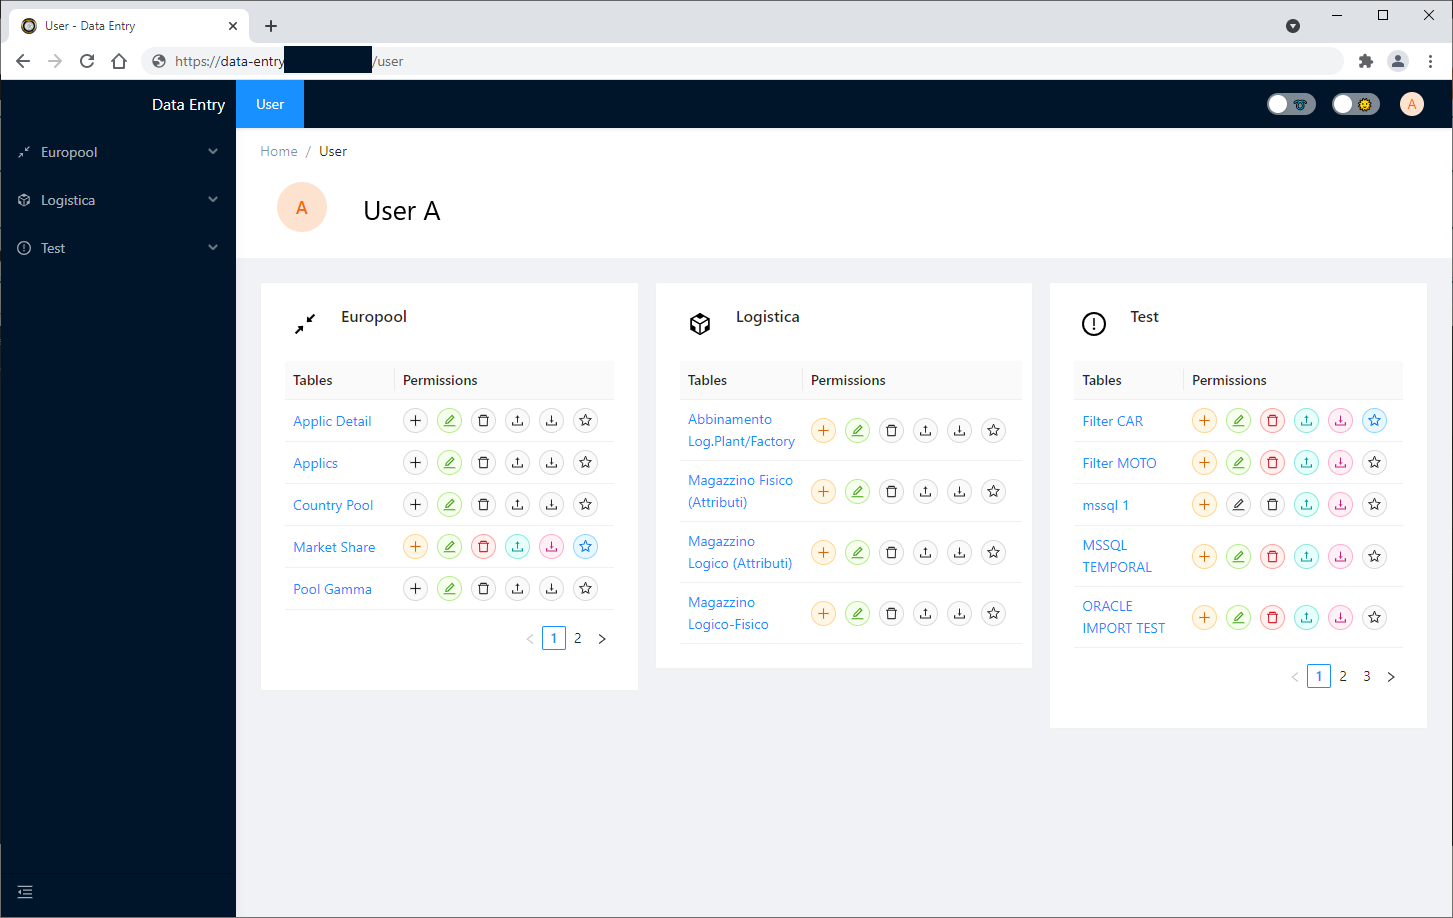
\includegraphics[width=15.8cm]{chapters/images/ch_3/FE/User/home_user.png}
    \caption{Users' homepage.}
    \label{fig:home}
\end{figure}

When the chosen table is opened, it needs to be built from scratch; for this purpose, all metadata of the table is retrieved from the Back-End and parsed to build it. This metadata contains:
\begin{itemize}
    \item the basic information of the table: the table name, the description, the collection it belongs to, and the executable action, if available;
    \item the permissions enabled for the user of the table, since the presence of action icons depends on them;
    \item all the visible fields of the table; each field contains the information needed to display the column properly, like the datatype or if it is possible to sort or filter by it, and the information to create the form for the insertion or update.
\end{itemize}

The result of the processing of these metadata can be seen in Figure \ref{fig:example}. In it we can see the actions enabled for the user in the upper part of the table and in the rightmost column, a fixed column on the left side of the table, with which one can only filter, and some columns with different datatype, with which one can filter and sort. Instead, in Figure \ref{fig:exampleEdit} we can see the form generated for inserting or updating a record; here are the fields available in display mode and those available for editing, each with their own datatype constraints.


\begin{figure}[!htb]
    \centering
    \begin{subfigure}{\linewidth}
        \centering
        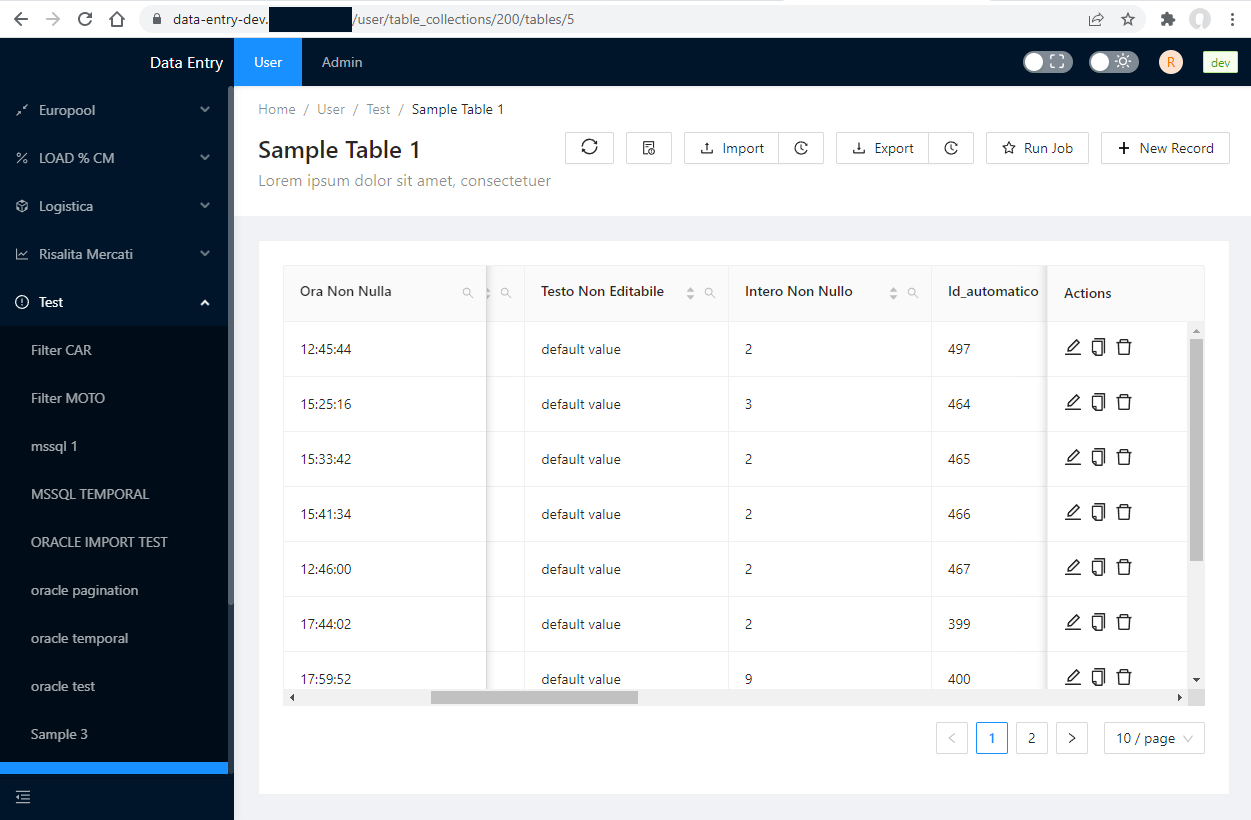
\includegraphics[width=14.5cm]{chapters/images/ch_3/FE/User/example.png}
        \caption{Example of a generated table.}
        \label{fig:example}
    \end{subfigure}
    \begin{subfigure}{\linewidth}
        \centering
        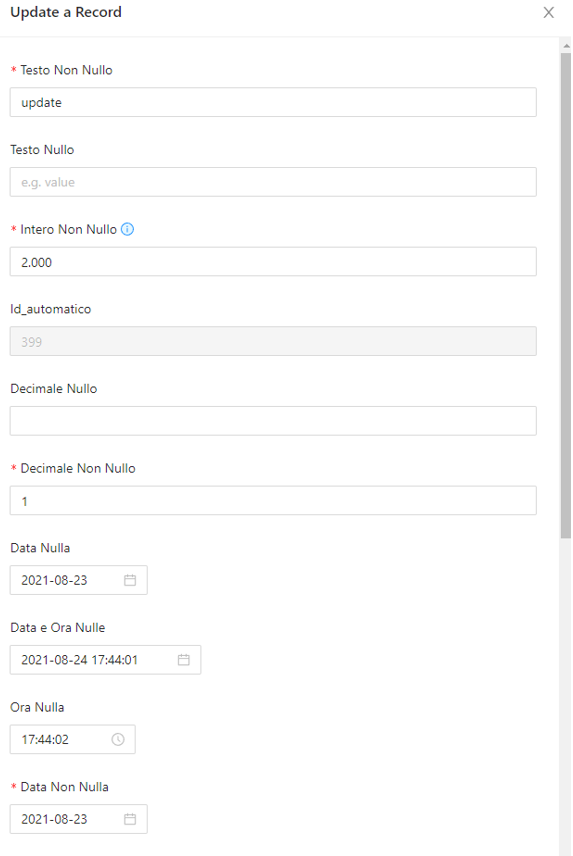
\includegraphics[width=8.5cm]{chapters/images/ch_3/FE/User/editExample.png}
        \caption{Example of a generated form.}
        \label{fig:exampleEdit}
    \end{subfigure}
    \caption{Result of the metadata processing.}
\end{figure}


\clearpage
\section{Deployment}
As mentioned earlier, the deployment of the tool is performed via GitLab's CI/CD tool, using a deployment pipeline for each branch. The pipeline execution depends on \emph{runners} provided by the company; a runner is an agent that runs the CI/CD jobs, where a job is a definition of what to do. Because the number of runners is limited, and knowing that the Data Entry Tool is not the only project in development for the client, we ran into difficulties because sometimes, in order to test a minor fix, we had to wait for a runner to become available, thus increasing the wait time between each deployment.  To this end I created a convention on the branch names and the pipeline executions.

\begin{table}[!htb]   
\small
  \centering
  \caption{Pipeline execution mode.}
  \begin{tabular}{|l|c|c|c|l|}
    \hline
    \textbf{Branch name} & \textbf{Environment} & \textbf{Automatic} & \textbf{Manual} & \textbf{Description}             \\\hline
    dev-*                & dev                  &                    & X               & Branches for feature development \\\hline
    dev                  & dev                  & X                  &                 & Main development branch          \\\hline
    master               & prod                 &                    & X               & Production release branch        \\\hline
  \end{tabular}
  
  \label{tab:pipe}
\end{table}

Table \ref{tab:pipe} represents the different execution mode of the pipelines depending on the branch: 

\begin{itemize}
    \item the only branch that would be automatically deployed through the pipeline was the \code{dev} branch, because it is the collection point for all completed features, allowing integration testing between new and existing features;
    \item  if the branch name starts with \code{dev-}, the pipeline for that branch must be manually triggered, because not every update on those branches implies a completed feature and we do not want to monopolize the available runners;
    \item the pipeline for the \code{master} branch has to be manually triggered, because its execution represents a release of a completed and tested set of features and we wanted full control on when the deploy started.
\end{itemize}


\subsection{Pipeline definition}
The pipeline used in each branch is divided into 4 phases, as shown in the figure \ref{fig:pipe}, and each phase represents the deployment of a section of the Data Entry Tool, and since each phase is independent of the other, it has been made so that each can be deployed independently by monitoring changes in their specific directory.

\begin{figure}[!htb]
  \centering
  \begin{tikzpicture}
    [
      grow                    = right,
      sibling distance        = 6em,
      level distance          = 4.5cm,
      edge from parent/.style = {draw, -latex},
      every node/.style       = {font=\footnotesize},
      sloped
    ]
    \node [env] {Schema Deploy}
    child { node [env] {Serverless Deploy}
        child { node [env] {Containers Deploy}
            child { node [env] {K8s Deploy} }
          }
      };
  \end{tikzpicture}
  \caption{Deployment pipeline steps.}
  \label{fig:pipe}
\end{figure}

\begin{enumerate}
    \item \textbf{Schema Deployment}: in this stage the schema of the database on which the tool work is updated. 
    \item \textbf{Serverless Deploy}: in this stage all the Back-End, meaning all the Lambdas, SQS queue, APIGateway, the encription keys, and sensitive keys, are deployed or updated via the Serverless Framework;
    \item \textbf{Containers Deploy}: this stage manages the creation and upload of a Docker container for the Front-End application;
    \item \textbf{K8s Deploy}: in this last stage the container created in the previous stage is taken and deployed via Rancher.
\end{enumerate}

\begin{figure}[!htb]
  \centering
  \tikzstyle{every node}=[draw=black,thick,anchor=west]
  \tikzstyle{folder}=[draw=blue,fill=blue!10]
  \tikzstyle{src}=[draw=green,fill=green!10]
  \begin{tikzpicture}[
      grow via three points={one child at (0.5,-0.7) and
          two children at (0.5,-0.7) and (0.5,-1.4)},
      edge from parent path={(\tikzparentnode.south) |- (\tikzchildnode.west)}]
    \node [folder] {\code{/} }
    child { node [folder]{\code{/db}}
        child {node [folder] {\code{/SQL}}            }
        child {node {\code{docker-compose.yml}}}
        child {node {\code{.gitlab-ci.yml}}}
      }
    child [missing] {}
    child [missing] {}
    child [missing] {}
    child { node [folder] {\code{/serverless}}
        child {node [src] {\code{/src}}}
        child {node {\code{.gitlab-ci.yml}}}
      }
    % child [missing] {}
    child [missing] {}
    child [missing] {}
    child { node [folder] {\code{/webapp}}
        child {node [src] {\code{/src}}}
        child {node {\code{.gitlab-ci.yml}}}
      }
    child [missing] {}
    child [missing] {}
    child { node [folder] {\code{/k8s}}
        child {node {\code{.gitlab-ci.yml}}}
      }
    child [missing] {}
    child {node {\code{.gitlab-ci.yml}}}
    ;
  \end{tikzpicture}
  \caption{Directory structure of the project.}
  \label{fig:directoryTree}
\end{figure}

From Figure \ref{fig:directoryTree} we can see an excerpt of the directory tree with the division into sections of the Data Entry Tool; each contains a file \code{.gitlab-ci.yml} including the definitions of both all the actions to be performed at the time of deployment, and the files to look at to start the specific stage of the pipeline. The \textbf{Containers Deploy} and \textbf{K8s Deploy} stages are tightly bound together because whenever there is an update on the Graphical User Interface, not only the container has to be recreated, but it has to be deployed via the orchestration system for it to be available for use.

\subsection{Schema Deploy}
The Aurora Instance at the heart of the project must exist before this phase of the pipeline is executed because, as shown in the Listing \ref{code:compose}, the Flyway command \code{migrate} needs a connection string to the database and the user and password used to perform operations on the specified schema.


\begin{lstlisting}[
    language=docker-compose-2, 
    caption={Docker-compose.yml used in the schema deployment.},
    breaklines=true,
    label={code:compose},
    captionpos=b
]
version: '3.9'
services:
    flyway:
        image: public.ecr.aws/XXXXXXXX/datamanagement/gitlab_ci/flyway/flyway:7.10-alpine
        command: -url=jdbc:postgresql://${DB_HOST_URL}:${DB_PORT}/data_entry
            -schemas=data_entry
            -user=${DB_USER}
            -password=${DB_PSW}
            migrate
        volumes:
            - ./SQL:/flyway/sql
\end{lstlisting}


The \code{migrate} command is an idempotent operation that scans the file-system for available migrations, in this case in the directory \code{/flyway/sql} where we mapped the content of the \code{/SQL} directory in the docker-compose file. After the scan, it will compare them to the migration previously applied to the database, and as shown in Figure \ref{fig:migrate}, if any difference is found, it will migrate the database to close the gap.

\begin{figure}[!htb]
    \centering
    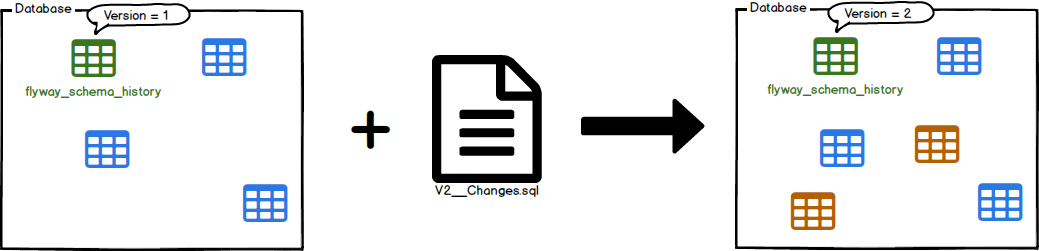
\includegraphics[ width = 15.5cm]{chapters/images/ch_3/command-migrate.png}
    \caption{Migration process.}
    \label{fig:migrate}
\end{figure}

\subsection{Serverless Deploy}
In this phase, the Back-End infrastructure is deployed using the Serverless Framework via AWS CloudFormation. For this purpose I created a custom docker image based on Alpine Linux, which was chosen because it has a small size. In the docker image I added Node v14, because it is the same version used in the Lambda's environment and the most recent version at the time of development, TypeScript, because it is the language chosen for development and is used to compile source code into JavaScript when the pipeline is running, and Serverless to deploy directly from the pipeline.

When this phase of the pipeline begins, the operations performed are:
\begin{enumerate}
    \item install all the dependencies;
    \item compile the TypeScript source code into JavaScript to be deployed in the Lambdas;
    \item copy of all the dependencies for the Lambda functions; 
    \item deploy of the infrastructure.
\end{enumerate}

\subsection{Containers Deploy}
For this phase, just like the Serverless Deploy phase, I created a custom Docker image, this time, in addition to Node v14, with the AWS Command Line Interface. Here the TypeScript source files are compiled into JavaScript via the AntDesign Pro specific build operation. Then the compiled files are copied into the Front-End container image, alongside the configuration files for NGINX, and uploaded to the client ECR instance with the help of the AWS CLI.


\subsection{K8s Deploy}
In this last phase, the information of the just created container image is used to create the Pod in the Rancher instance. To do so, the operations performed are:
\begin{enumerate}
    \item creation of the Pod, by using the Front-End container image;
    \item exposition of the listening port 80 of the Pod and binding of the API gateway. In this way the Back-End APIs are reachable from the Pod;
    \item binding of the Pod listening port 80 to the Ingress port 80, exposition of the Tool URL to be reachable from the client, and addition of the TLS certificate to ensure secure data exchange.
\end{enumerate}


% \clearpage
\section{Implementation}
% 3.3  Aspetti implementativi  (qui non deve commentare tutto il codice, ma solo descrivere gli aspetti più importanti o problematici del lavoro, evidenziando come ha affrontato i problemi o che idee originali ha avuto nello sviluppo.  Poche righe di codice se e solo se proprio le servono per spiegare qualcosa che ha fatto.)

   
In this next section, I will convey the most important implementation aspects of the creation of the Data Entry Tool.

\subsection{Multiple Database Governance}
\subsubsection{Interacting with different databases} \label{Knex}
%-> knex con i multi db, usato perchè non serve un orm essendo dinamico
One of the challenges I had to deal with was having to manage more than one database at a time. All databases are different from one another, because of the DBMS used, the very different structure of the tables that exist in those databases, or the different Entity-Relationship schemas that they have to manage. This is one of the reasons I did not use an Object-Relational Mapping; this kind of technique makes it possible to query and manipulate data from a database using an object-oriented paradigm; however, to do so it is needed to know in advance the underlying data structure of the tables it tries to manipulate. With the Data Entry Tool this is not possible since the databases, or the tables that reside there, are not known in advance. Another reason not to use an ORM library is that there is no library in TypeScript that can handle all the required DBMSs at the same time.

With the ORM out of the equation, I had to find another solution to handle the databases. Fortunately, I found Knex.js \cite{knex}, an SQL query builder that allows to create queries via method chaining, shown in Code Sample \ref{code:knex}, has transaction support, and works with all the required DBMSs. The ability to build a query through method chaining made it possible to create different queries based on the execution flow.

\begin{lstlisting}[
    language=typescript,
    caption={Example of query creation with Knex.},
    breaklines=true,
    label={code:knex},
    captionpos=b
]
import knex from 'knex'

const db = knex(...)

db.select(...)
    .from(...)
    .where(...)
\end{lstlisting}

Knex uses the parameters provided when a database is first added to the Tool, i.e. the database name, connection host and port, database user and password, to establish a connection and perform operations on it. 
However, since establishing a connection takes time, whenever a user has to perform an operation on a database, after creating the connection, I cache it in a dictionary. 
This is done to follow the temporal locality principle: if a user needs to perform an operation on a given table in a given database, then s/he is likely to perform other operations on that particular table in the near future.
This way, any user who needs to access that database, even if for a different table, does not have to establish a new connection to perform operations. Moreover, any operation performed on any database registered in the Tool, or on the Aurora instance on which it is based, is performed through a transaction. This is done to prevent any concurrency while interacting with the data, given the dynamic nature of the databases and their distributed access.


\subsubsection{Automatic column retrieval}
When a new table is added to the Tool, it starts the process of automatic column retrieval. This process is done to save the user the tedious work of manually inserting all the columns of a table. However, since different DBMSs have different places where they store the metadata for each table, I had to create custom queries to retrieve the data. 

Fortunately, both PostgreSQL and Microsoft SQL Server use the same set of tables, but OracleDB uses a different set, as displayed in Table \ref{tab:tables}.

\begin{table}[!htb]   
\small
  \centering
  \caption{Tables containing metadata.}
  \begin{tabular}{|l|l|ll|}\hline
    Engine                    & Schema                               &             & Tables             \\\hline
    PostgreSQL                & \multirow{3}{*}{information\_schema} & \textbullet & columns            \\
    Microsoft SQL SERVER      &                                      & \textbullet & table\_constraints \\
                              &                                      & \textbullet & key\_column\_usage \\\hline
    \multirow{3}{*}{OracleDB} & \multirow{3}{*}{SYS}                 & \textbullet & ALL\_TAB\_COLUMNS  \\
                              &                                      & \textbullet & ALL\_CONSTRAINTS   \\
                              &                                      & \textbullet & ALL\_CONS\_COLUMNS \\
    \hline
  \end{tabular}
  \label{tab:tables}
\end{table}

Through the process of table joining, with the original name and schema of the new table added as background information, it is possible to get the elements that make up a column, or at least the set of essential information. This set consists of:
\begin{itemize}
    \item knowing whether a column is a primary key;
    \item knowing whether the column can have empty/null values;
    \item knowing if the column can be modified. This is done by checking if it is a primary key and if it has a default value;
    \item the data type of the column. Since we cannot use all the possible data types available in all the DBMSs, the column data type is mapped to a generic data type that represents it. The data types available in this automatic process are:
    \begin{itemize}
        \item BOOLEAN
        \item STRING
        \item NUMERIC
        \item DATE
        \item TIME
        \item DATETIME
    \end{itemize}
\end{itemize}

\subsubsection{A View to ease information retrieval}
The information regarding the association between a user and a table is spread across many tables. This means that, in order to reach the metadata of a table, given a user, many tables must be traversed, and doing so each time would have made the source code difficult to read and debug in case of problems. For this reason, I created a view that gathers in one place the essential information needed to retrieve metadata, to check a user's permissions, to correctly display a table, and to connect to the original database to perform operations.

Regarding permissions on a table, since a user can have access to one across multiple user groups, it makes sense to always enable the sum of permissions on that table regardless of where they access the table. For this purpose, the view contains a sub-query, visible in Code Sample \ref{code:view}, which performs an aggregation based on the username and the associated table. With it and the aggregation function \code{bool\_or()}, it is possible to perform the logical addition of the permissions present in a user group for a given table accessible to a given user. In addition, an aggregation is done on the table fields, more precisely to check if among the fields of a table there is also one marked as primary key. This is necessary to prevent a user from trying to update or delete a record in a table where a primary key is not defined. Otherwise, when deleting or updating using the \code{where} condition, all elements that satisfy the condition are manipulated. 

\begin{lstlisting}[ 
    language=sql,
    caption={Sub-query of the view.},
    breaklines=true,
    label={code:view},
    captionpos=b
]
WITH users_tables_agg AS (
    SELECT
        u.username,
        ugt.table_id,
        bool_or(ugt.can_insert) AS can_insert,
        bool_or(ugt.can_update) AS can_update,
        bool_or(ugt.can_delete) AS can_delete,
        bool_or(ugt.can_import) AS can_import,
        bool_or(ugt.can_export) AS can_export,
        bool_or(ugt.can_perform_action) AS can_perform_action,
        bool_or(ugt.can_batch_delete) AS can_batch_delete,
        bool_or(tf.primary_key) AS has_primary_key
    FROM
        users u
    JOIN users_user_groups uug ON
        u.username = uug.username
    JOIN user_groups_tables ugt ON
        uug.group_id = ugt.group_id
    LEFT JOIN table_fields tf ON 
        ugt.table_id = tf.table_id 
    GROUP BY
        u.username,
        ugt.table_id
 )
\end{lstlisting}

This view, however, is not a materialized view. The reason is that, since metadata is very dynamic, pre-computing a materialized view, and keeping it up-to-date, would take more time than would be saved by using it, since it has to be updated every time an element in the view changes.

\subsubsection{The Filtering conundrum} 
% vengono usate strutture generiche perchè non sapevamo a priori le colonne che si sarebbero usate
In both the Administrator and User views of the Data Entry Tool, it is possible to filter the elements of a table according to the values of one or more columns. For the Administrator side, the columns to filter are predefined and never change; however the same cannot be said for the User side. On their side, the tables are dynamically generated and do not always reflect the structure present of their source databases. Just as the structure is dynamic, the number and type of columns to filter for is dynamic as well. Therefore, it was necessary to create a flexible and easy-to-use way to represent a filter. For this reason, I created a filter type with a structure that could be easily used by both the Administrator and User side with Knex's query building capabilities.

\begin{lstlisting}[ 
    language=typescript,
    caption={Composition of a filter.},
    breaklines=true,
    label={code:filter},
    captionpos=b
]
type Filter = {
    operation: Operations
    column: string
    toCompare: unknown | [unknown, unknown] | Array<unknown>
}
\end{lstlisting}

In the Code Sample \ref{code:filter}, we can see that a filter consists of an operation, described in Table \ref{tab:filtering}, the name of the column to be filtered, and a comparison element represented by a union type. A \emph{Union Type} describes a value that can be one of several types. Since it is not possible to know a priori the actual type of the element of comparison used in the process of filtering, this Union Type conceptually represents the number of elements for which to compare the values of a column. The represented types are, in order:
\begin{itemize}
    \item \emph{unknown}: this type represents a single value that can be used with comparison operations, i.e. greater than, equal, or similar to a value in the given column. This representation is used by columns that contains numbers, boolean, or alphanumeric strings.
    \item \emph{[unknown, unknown]}: this type represents a range used to check if a value in the given column belongs to it or not. This representation is used by columns that contains numbers or temporal data.
    \item \emph{Array$<$unknown$>$}: a generalized version of the previous type that is used by columns with alphanumeric values.
\end{itemize}


\subsection{Serverless management} 
\subsubsection{Lambda's environment}%-> gestione dei layer con ottimizzazione del caricamento dei layer sulle Lambda
When building Serverless applications, it is quite common to have code that is shared between Lambda functions. This can be custom code, which is used by more than one function, or a standard library, which is used to simplify the implementation of the business logic. Instead of adding the dependencies to each Lambda, effectively increasing the storage size that they will use and the time needed to deploy a function, it is possible to centralize all the common dependencies they will use. A \emph{Lambda Layer} is an archive that can contain libraries, a custom runtime environment, data, or configuration files. When a layer is included in a function, the content is extracted from the archive and used in the execution environment.

For the creation of the Lambda functions for the Data Entry Tool, I created two different layers, shown in Code Sample \ref{code:layer}.


\begin{lstlisting}[
    language=sls,
    caption={Layers defined in the project.},
    breaklines=true,
    label={code:layer},
    captionpos=b
]
nodeModulesLayer: 
    path: layers/layer_node_modules
    name: nodeModulesLayer
    description: Node Modules Layer

oracleClientLayer: 
    path: layers/oracle_client
    name: oracleClientLayer
    description: Oracle Client Layer to manage database connection
\end{lstlisting}

The first layer, \emph{nodeModulesLayer}, consists of all NodeJs dependencies used in all Lambda functions; since OracleDB is a proprietary DBMS, a specific client is needed to access it, and so the second layer, \emph{oracleClientLayer}, is the client that is used to access it. However, for security reasons, only a small number of Lambda functions can use this layer.

With these layers, the average size of a Lambda function drops from 70MiB to 15KiB.


\subsubsection{API Gateway naming problem}
%-> con cloud formation la risoluzione del nome di apiGatewayDeployment
While developing the Serverless infrastructure, I discovered an issue regarding the definition of the API Gateway. Since OpenAPI is used to define the APIs used in the Back-End side, each time the API definition is updated, a new Back-End deployment must be performed. However, the deployment failed as the existing API Gateway was updated in place. To get around this problem, I created a script that runs during the Serverless Deploy step of the pipeline. The purpose of this script is to read the configuration file where the API Gateway is defined, and change the resource name that is being created by adding the deployment timestamp at the end of it. This way, the created resource is always ``new'', and the deployed one will be destroyed.


\subsection{Front-End}
 %-> FE parte user che è dinamica (es metadati per la generazione della pagina dinamica, catalogazione dei tipi custom)
\subsubsection{Standardize the experience}
Because the Administrator side of the Front-End has a static interface, meaning that it does not change amongst users who use it, many similar components can be reused with little or no change throughout the web application. Moreover, some elements can be reused in the end user side as well. 

The main actions available with every table, i.e., insert, update, delete, and duplicate a row, are parameterized components and agnostic to the tables they must manage. While the actions of paging, sorting and filtering have only a common basic structure, but their functioning depends more strictly on the tables that use them.

For the administrator side, there are 4 sections whose behavior is more or less the same, namely pages for table collections, databases, tables and fields. Each one has a table with a specific number of columns and a form for the insertion or update of a row. For these pages, I created templates for the table and the form to facilitate their development, since what needs to change is the number of columns and the endpoint from which to retrieve them.

The end user side is very dynamic since it must adapt the interface according to the user. For this reason, it is not possible to use a predefined template such as a ``silver bullet'' for the construction of all possible tables. Therefore, their creation depends on the metadata received from the Back-End. As mentioned before, this metadata contains, other than the actual table information and list of permissions, the list of fields retrieved from the table ``\code{Table Fields}''; after removing all the fields that are not visible, those that remain are mapped to the table columns by checking the data type, applying the badges for filtering and sorting, and finally sorted in the order decided by the administrator.


